% Автоматаар үүсгэсэн — эх файл: lab02/README.md
\chapter{Лаб 2 — Төхөөрөмжийн бүрэн амьдралын мөчлөг ба OTA}

\begingroup\scriptsize\begin{longtable}[]{@{}
  >{\raggedright\arraybackslash}p{(\columnwidth - 2\tabcolsep) * \real{0.5000}}
  >{\raggedright\arraybackslash}p{(\columnwidth - 2\tabcolsep) * \real{0.5000}}@{}}
\toprule
\endhead
\bottomrule
\endlastfoot
\textbf{7 хоног} & V \\
\textbf{Хугацаа} & 4 цаг \\
\textbf{Суралцахуйн үр дүн} & ҮД4 (аюулгүй төхөөрөмж, өгөгдлийн удирдлага) \\
\textbf{Үнэлгээ} & Бичгийн тайлан, 10 оноо \\
\textbf{Гол хэмжилт} & Бүртгэлийн хурд, OTA-гийн хугацаа ба амжилтын хувь \\
\end{longtable}\endgroup

\hypertarget{ux437ux43eux440ux438ux43bux433ux43e}{%
\section{1. Зорилго}\label{ux437ux43eux440ux438ux43bux433ux43e}}

Төхөөрөмжийн амьдралын мөчлөгийн \textbf{дөрвөн үе шатыг} өөрсдөө хэрэгжүүлж, хэмжинэ:

\begin{verbatim}
бүртгэл (provisioning) → таних тэмдэг (identity) → OTA шинэчлэлт → хүчингүй болгох (revocation)
\end{verbatim}

Худалдааны платформууд (ThingsBoard, AWS IoT, Azure IoT Hub) эдгээрийг \textbf{хар хайрцаг} болгож нуудаг. Энэ лабораторид та \texttt{lab02/\allowbreak{}registry/\allowbreak{}app.\allowbreak{}py} (≈500 мөр) ба \texttt{lab02/\allowbreak{}ota\_\allowbreak{}agent.\allowbreak{}py} (≈270 мөр) хоёрыг \textbf{уншиж, ажиллуулж, эвдэж} протоколыг ил харна.

\begin{quote}
\textbf{Яагаад ThingsBoard биш вэ:} ThingsBoard-ын албан ёсны заавар хөгжүүлэлт/PoC-д хүртэл 4 GB RAM шаарддаг. Pi 3B-д нийт 1 GB (OS-д \textasciitilde925 MiB). Гэхдээ илүү чухал шалтгаан бий --- та энэ хичээлээр \emph{платформ ашиглагч} биш \emph{платформ зохиогч} болох ёстой. Лабораторийн эцэст сонголтот харьцуулалт хийнэ (§4, Алхам 8).
\end{quote}

\hypertarget{ux443ux440ux44cux434ux447ux438ux43bux441ux430ux43d-ux43dux4e9ux445ux446ux4e9ux43b}{%
\section{2. Урьдчилсан нөхцөл}\label{ux443ux440ux44cux434ux447ux438ux43bux441ux430ux43d-ux43dux4e9ux445ux446ux4e9ux43b}}

\begin{itemize}
\tightlist
\item
  Лаб 1 дууссан, \texttt{lab01-done} tag тавигдсан
\item
  {[}ЗК{]} \texttt{cd\ stack\ \&\allowbreak{}\&\allowbreak{}\ make\ up\ \&\allowbreak{}\&\allowbreak{}\ make\ health} → бүх мөр 200
\item
  {[}Pi{]} \texttt{cd\ edge\ \&\allowbreak{}\&\allowbreak{}\ make\ up\ \&\allowbreak{}\&\allowbreak{}\ make\ link} → \texttt{bridge/state\ 1}
\item
  Бие даалт IV: X.509 сертификатын гинжин хэлхээ (CA → төхөөрөмж) уншсан
\end{itemize}

\begin{Shaded}
\begin{Highlighting}[]
\CommentTok{\# [ЗК] бүртгэлийн үйлчилгээ ажиллаж байгаа эсэх}
\ExtensionTok{curl} \AttributeTok{{-}s}\NormalTok{ localhost:8090/health }\KeywordTok{|} \ExtensionTok{jq}
\CommentTok{\# → \{"ok": true, "devices": 0, "mqtt": true\}}
\end{Highlighting}
\end{Shaded}

\hypertarget{ux43eux43dux43eux43bux44bux43d-ux441ux430ux43dux443ux443ux43bux433ux430}{%
\section{3. Онолын сануулга}\label{ux43eux43dux43eux43bux44bux43d-ux441ux430ux43dux443ux443ux43bux433ux430}}

\hypertarget{bulk-vs-jit-ux445ux43eux451ux440-ux437ux430ux433ux432ux430ux440ux44bux43d-ux441ux43eux43bux438ux43bux446ux43eux43e}{%
\subsection{Bulk vs JIT --- хоёр загварын солилцоо}\label{bulk-vs-jit-ux445ux43eux451ux440-ux437ux430ux433ux432ux430ux440ux44bux43d-ux441ux43eux43bux438ux43bux446ux43eux43e}}

\begingroup\scriptsize\begin{longtable}[]{@{}
  >{\raggedright\arraybackslash}p{(\columnwidth - 4\tabcolsep) * \real{0.3333}}
  >{\raggedright\arraybackslash}p{(\columnwidth - 4\tabcolsep) * \real{0.3333}}
  >{\raggedright\arraybackslash}p{(\columnwidth - 4\tabcolsep) * \real{0.3333}}@{}}
\toprule
\begin{minipage}[b]{\linewidth}\raggedright
\end{minipage} & \begin{minipage}[b]{\linewidth}\raggedright
\textbf{Bulk (бөөнөөр)}
\end{minipage} & \begin{minipage}[b]{\linewidth}\raggedright
\textbf{JIT (яг цагт нь)}
\end{minipage} \\
\midrule
\endhead
\bottomrule
\endlastfoot
Хэзээ бүртгэнэ & үйлдвэрээс гарахаас өмнө & төхөөрөмж анх залгагдахад \\
Нэвтрэлт хаанаас & урьдчилан үүсгэж бүтээгдэхүүнд суулгана & төхөөрөмж өөрөө гуйна \\
Давуу тал & хяналттай, аудит хийхэд амархан & ашиглагдаагүй бүртгэл үлдэхгүй \\
Сул тал & 10 000 бүртгэлээс 3 000 нь хэзээ ч ашиглагдахгүй & \textbf{хэн болохыг батлах} асуудал хурцаар тавигдана \\
Хэзээ хэрэглэх & хаалттай флот, тодорхой тоо & нээлттэй тархалт, тодорхойгүй тоо \\
\end{longtable}\endgroup

JIT-ийн гол эрсдэл: баталгаагүй бол \textbf{хэн ч} \texttt{device\_id} сонгоод флотод нэвтэрч болно. Шийдэл нь үйлдвэрт суусан X.509 сертификат --- үүнийг Алхам 3-т хийнэ.

\hypertarget{ux442ux430ux43dux438ux445-ux442ux44dux43cux434ux433ux438ux439ux43d-ux433ux443ux440ux432ux430ux43d-ux442ux4afux432ux448ux438ux43d}{%
\subsection{Таних тэмдгийн гурван түвшин}\label{ux442ux430ux43dux438ux445-ux442ux44dux43cux434ux433ux438ux439ux43d-ux433ux443ux440ux432ux430ux43d-ux442ux4afux432ux448ux438ux43d}}

\begingroup\scriptsize\begin{longtable}[]{@{}llll@{}}
\toprule
Түвшин & Механизм & Хулгайлагдвал & Хэрэглээ \\
\midrule
\endhead
\bottomrule
\endlastfoot
1 & нэр/нууц үг & бүх флот эрсдэлд & зөвхөн лаборатори \\
2 & төхөөрөмж тус бүрийн токен & нэг төхөөрөмж & дунд зэрэг \\
3 & \textbf{X.509 + mTLS} & нэг төхөөрөмж, CRL-ээр хаана & үйлдвэрлэл \\
\end{longtable}\endgroup

\hypertarget{ota-ux433ux438ux439ux43d-ux43fux440ux43eux442ux43eux43aux43eux43b-cnc302-ux445ux443ux432ux438ux43bux431ux430ux440}{%
\subsection{OTA-гийн протокол --- CNC302 хувилбар}\label{ota-ux433ux438ux439ux43d-ux43fux440ux43eux442ux43eux43aux43eux43b-cnc302-ux445ux443ux432ux438ux43bux431ux430ux440}}

\begin{verbatim}
сервер → төхөөрөмж   .../ota/offer     {fw_id, version, size, sha256, chunk_size, chunks}
төхөөрөмж → сервер   .../ota/request   {fw_id, chunk: N}
сервер → төхөөрөмж   .../ota/chunk/N   <хоёртын 4 KiB>
төхөөрөмж → сервер   .../ota/state     {state, progress, error}
\end{verbatim}

\begin{figure}
\centering
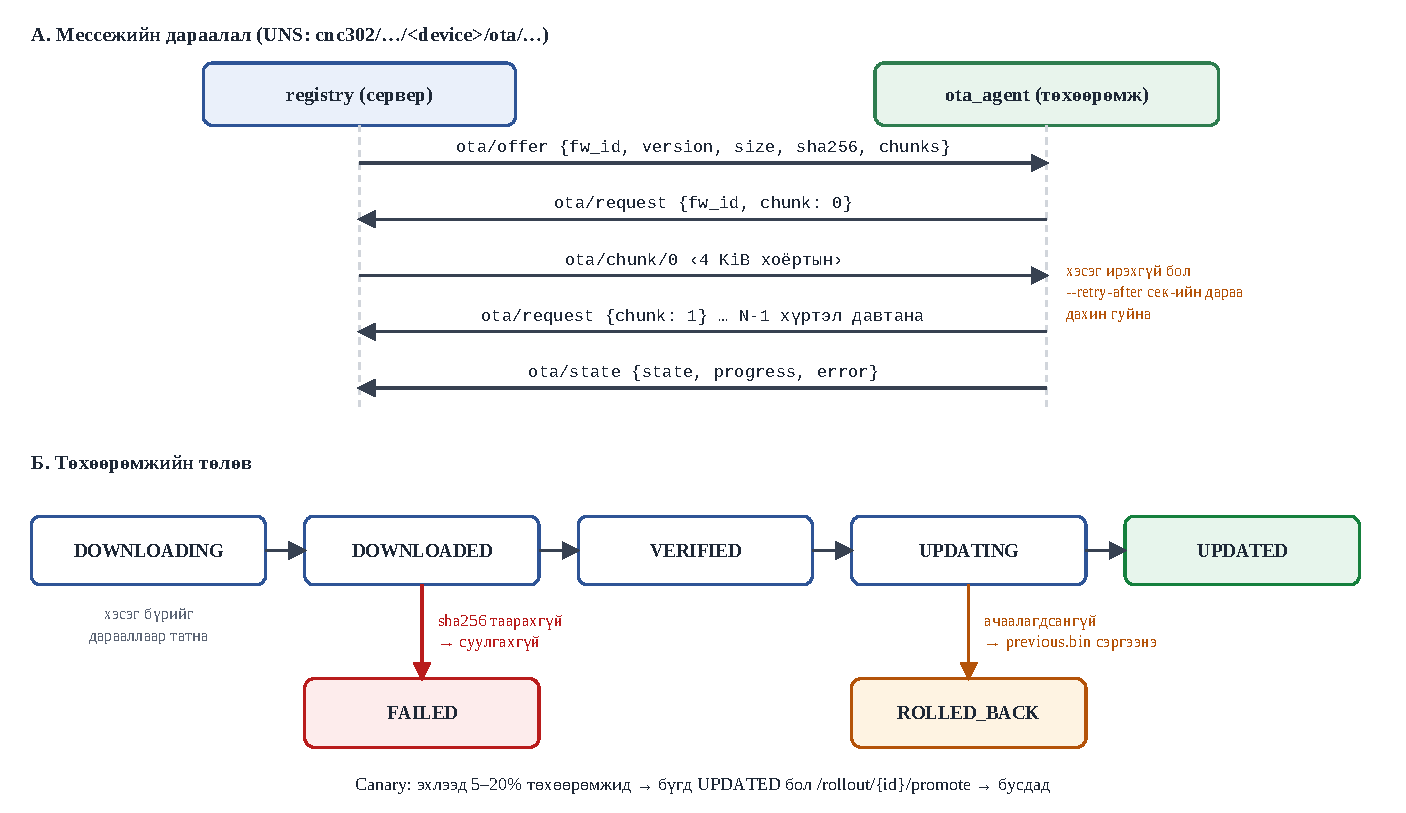
\includegraphics{figures/fig-ota-states.pdf}
\caption{Зураг 2.1 --- OTA-гийн төлөвийн машин ба MQTT мессежийн дараалал (offer → request → chunk/N → state)}
\end{figure}

Төлөвийн дараалал:

\begin{verbatim}
DOWNLOADING → DOWNLOADED → VERIFIED → UPDATING → UPDATED
                               ↓            ↓
                            FAILED     ROLLED_BACK
\end{verbatim}

\textbf{Гурван зүйл заавал байх ёстой}, эс бөгөөс OTA нь тоосго үйлдвэрлэх машин болно:

\begin{enumerate}
\def\labelenumi{\arabic{enumi}.}
\tightlist
\item
  \textbf{Шалгах (checksum).} Татсан файл эвдэрсэн эсэхийг суулгахаас ӨМНӨ шалгана.
\item
  \textbf{Буцаах (rollback).} Шинэ хувилбар ачаалагдахгүй бол хуучинд буцна. Тиймээс A/B хуваалт эсвэл нөөц хуулбар хэрэгтэй.
\item
  \textbf{Canary.} 5 000 төхөөрөмжийг нэг дор шинэчилж эвдвэл засах арга байхгүй. Эхлээд 5--20\%-д, амжилттай бол бусдад.
\end{enumerate}

\hypertarget{ux430ux43bux445ux43cux443ux443ux434}{%
\section{4. Алхмууд}\label{ux430ux43bux445ux43cux443ux443ux434}}

\hypertarget{ux430ux43bux445ux430ux43c-0-emqx-rest-api-ux442ux4afux43bux445ux4afux4afux440-ux431ux430-authenticator-15-ux43cux438ux43d-ux437ux43a}{%
\subsection{Алхам 0 --- EMQX REST API түлхүүр ба authenticator (15 мин) {[}ЗК{]}}\label{ux430ux43bux445ux430ux43c-0-emqx-rest-api-ux442ux4afux43bux445ux4afux4afux440-ux431ux430-authenticator-15-ux43cux438ux43d-ux437ux43a}}

\texttt{registry} нь EMQX-ийн REST API-г (\texttt{/api/v5}) дуудаж төхөөрөмж бүрд MQTT нэвтрэлт үүсгэнэ. REST API нь \textbf{самбарын admin нууц үгийг хүлээн авдаггүй} (EMQX 5.0-оос хойш) --- зөвхөн API key / secret key-г HTTP Basic нэвтрэлтээр хүлээн авна.

\begin{enumerate}
\def\labelenumi{\arabic{enumi}.}
\item
  http://localhost:18083 → \textbf{System → API Key → + Create} → Expire At хоосон → \textbf{Confirm}. Secret key-г \textbf{тэр дор нь} хуулж ав --- дахин харагдахгүй.
\item
  \texttt{stack/.env}-д бичээд \texttt{registry}-г шинэ утгатай нь дахин үүсгэ:

\begin{Shaded}
\begin{Highlighting}[]
\BuiltInTok{cd}\NormalTok{ \textasciitilde{}/cnc302/stack}
\FunctionTok{nano}\NormalTok{ .env                         }\CommentTok{\# EMQX\_API\_KEY=…  EMQX\_API\_SECRET=…}
\ExtensionTok{docker}\NormalTok{ compose }\AttributeTok{{-}{-}profile}\NormalTok{ core up }\AttributeTok{{-}d}\NormalTok{ registry}
\BuiltInTok{export} \VariableTok{EMQX\_API\_KEY}\OperatorTok{=}\VariableTok{$(}\FunctionTok{grep} \StringTok{\textquotesingle{}\^{}EMQX\_API\_KEY=\textquotesingle{}}\NormalTok{ .env }\KeywordTok{|} \FunctionTok{cut} \AttributeTok{{-}d}\OperatorTok{=} \AttributeTok{{-}f2}\VariableTok{)}
\BuiltInTok{export} \VariableTok{EMQX\_API\_SECRET}\OperatorTok{=}\VariableTok{$(}\FunctionTok{grep} \StringTok{\textquotesingle{}\^{}EMQX\_API\_SECRET=\textquotesingle{}}\NormalTok{ .env }\KeywordTok{|} \FunctionTok{cut} \AttributeTok{{-}d}\OperatorTok{=} \AttributeTok{{-}f2}\VariableTok{)}
\ExtensionTok{curl} \AttributeTok{{-}s} \AttributeTok{{-}u} \StringTok{"}\VariableTok{$EMQX\_API\_KEY}\StringTok{:}\VariableTok{$EMQX\_API\_SECRET}\StringTok{"}\NormalTok{ localhost:18083/api/v5/nodes }\KeywordTok{|} \ExtensionTok{jq} \StringTok{\textquotesingle{}.[0].version\textquotesingle{}}
\CommentTok{\# → "5.8.6"}
\end{Highlighting}
\end{Shaded}
\item
  \textbf{Built-in database} authenticator-ыг \textbf{идэвхгүй} (\texttt{"enable":\ false}) байдлаар үүсгэнэ. Үүсгээгүй бол хэрэглэгч нэмэх дуудлага \texttt{404\ Authenticator\ not\ found} буцаана. Идэвхгүй үед ч хэрэглэгч нэмэх боломжтой; харин EMQX нээлттэй хэвээр үлдэж, гүүр ба бусад клиент тасрахгүй. Алхам 7-д л идэвхжүүлнэ.

\begin{Shaded}
\begin{Highlighting}[]
\ExtensionTok{curl} \AttributeTok{{-}s} \AttributeTok{{-}u} \StringTok{"}\VariableTok{$EMQX\_API\_KEY}\StringTok{:}\VariableTok{$EMQX\_API\_SECRET}\StringTok{"} \AttributeTok{{-}X}\NormalTok{ POST localhost:18083/api/v5/authentication }\DataTypeTok{\textbackslash{}}
  \AttributeTok{{-}H} \StringTok{\textquotesingle{}content{-}type: application/json\textquotesingle{}} \DataTypeTok{\textbackslash{}}
  \AttributeTok{{-}d} \StringTok{\textquotesingle{}\{"mechanism":"password\_based","backend":"built\_in\_database",}
\StringTok{       "user\_id\_type":"username",}
\StringTok{       "password\_hash\_algorithm":\{"name":"sha256","salt\_position":"suffix"\},}
\StringTok{       "enable":false\}\textquotesingle{}} \KeywordTok{|} \ExtensionTok{jq} \StringTok{\textquotesingle{}.id, .enable\textquotesingle{}}
\CommentTok{\# → "password\_based:built\_in\_database"  false}
\end{Highlighting}
\end{Shaded}
\end{enumerate}

\begin{quote}
⚠ EMQX-ийн баримтаар authenticator идэвхтэй үед нэвтрэлтийн мэдээлэл нь олдоогүй клиент (сүүлийн authenticator дээр) \textbf{татгалзагдана} --- нэр/нууц үггүй бүх клиент ч мөн адил. Иймээс authenticator-ыг зөвхөн Алхам 7-д богино хугацаанд асаана.

Албан ёсны баримт: \href{https://docs.emqx.com/en/emqx/v5.8/guides/api.html}{EMQX REST API} · \href{https://docs.emqx.com/en/emqx/v5.8/guides/api-keys.html}{API Keys} · \href{https://docs.emqx.com/en/emqx/v5.8/guides/access-control/authn/authn.html}{Authentication} · \href{https://docs.emqx.com/en/emqx/v5.8/guides/access-control/authn/mnesia.html}{Built-in Database}
\end{quote}

\hypertarget{ux430ux43bux445ux430ux43c-1-bulk-ux431ux4afux440ux442ux433ux44dux43b-ux431ux430-ux445ux443ux440ux434ux43dux44b-ux445ux44dux43cux436ux438ux43bux442-30-ux43cux438ux43d-ux437ux43a}{%
\subsection{Алхам 1 --- Bulk бүртгэл ба хурдны хэмжилт (30 мин) {[}ЗК{]}}\label{ux430ux43bux445ux430ux43c-1-bulk-ux431ux4afux440ux442ux433ux44dux43b-ux431ux430-ux445ux443ux440ux434ux43dux44b-ux445ux44dux43cux436ux438ux43bux442-30-ux43cux438ux43d-ux437ux43a}}

\begin{Shaded}
\begin{Highlighting}[]
\BuiltInTok{cd}\NormalTok{ \textasciitilde{}/cnc302/lab02}
\ExtensionTok{python3}\NormalTok{ provision.py bulk }\AttributeTok{{-}{-}count}\NormalTok{ 10  }\AttributeTok{{-}{-}out}\NormalTok{ out/devices.csv}
\ExtensionTok{python3}\NormalTok{ provision.py bulk }\AttributeTok{{-}{-}count}\NormalTok{ 100 }\AttributeTok{{-}{-}prefix}\NormalTok{ b100 }\AttributeTok{{-}{-}out}\NormalTok{ out/b100.csv}
\ExtensionTok{python3}\NormalTok{ provision.py bulk }\AttributeTok{{-}{-}count}\NormalTok{ 500 }\AttributeTok{{-}{-}prefix}\NormalTok{ b500 }\AttributeTok{{-}{-}out}\NormalTok{ out/b500.csv}
\ExtensionTok{python3}\NormalTok{ provision.py list }\AttributeTok{{-}{-}limit}\NormalTok{ 10}
\end{Highlighting}
\end{Shaded}

\hypertarget{ux445ux4afux441ux43dux44dux433ux442-2.1-bulk-ux431ux4afux440ux442ux433ux44dux43bux438ux439ux43d-ux445ux443ux440ux434}{%
\subsubsection{Хүснэгт 2.1 --- Bulk бүртгэлийн хурд}\label{ux445ux4afux441ux43dux44dux433ux442-2.1-bulk-ux431ux4afux440ux442ux433ux44dux43bux438ux439ux43d-ux445ux443ux440ux434}}

\begingroup\scriptsize\begin{longtable}[]{@{}llll@{}}
\toprule
Төхөөрөмжийн тоо & Нийт хугацаа (сек) & мс/төхөөрөмж & Тэмдэглэл \\
\midrule
\endhead
\bottomrule
\endlastfoot
10 & & & \\
100 & & & \\
500 & & & \\
\end{longtable}\endgroup

\begin{quote}
Хугацаа \textbf{шугаман} өсөж байна уу? Үгүй бол хаана бөглөрч байна вэ? (Санамж: \texttt{app.py}-ийн \texttt{bulk()} бүх INSERT-ийг НЭГ transaction-д хийдэг, харин төхөөрөмж бүрд EMQX руу нэг HTTP дуудлага (\texttt{emqx\_\allowbreak{}add\_\allowbreak{}user}) явуулдаг. \texttt{EMQX\_\allowbreak{}API\_\allowbreak{}KEY}-гүйгээр ажиллуулж харьцуул.)

\texttt{devices.csv}-ийн \texttt{emqx} багана \texttt{created} байх ёстой. \texttt{skipped} бол Алхам 0-ийн 2-р хэсэг, \texttt{error\ 404} бол 3-р хэсэг хийгдээгүй.
\end{quote}

⚠ \texttt{out/devices.csv} нь нууц үг агуулна. \texttt{.gitignore}-д байгааг батал:

\begin{Shaded}
\begin{Highlighting}[]
\FunctionTok{git}\NormalTok{ check{-}ignore }\AttributeTok{{-}v}\NormalTok{ lab02/out/devices.csv    }\CommentTok{\# мөр буцаах ЁСТОЙ}
\end{Highlighting}
\end{Shaded}

\hypertarget{ux430ux43bux445ux430ux43c-2-jit-ux431ux4afux440ux442ux433ux44dux43b-ux431ux430-ux442ux4afux4afux43dux438ux439-ux44dux43cux437ux44dux433-ux431ux430ux439ux434ux430ux43b-20-ux43cux438ux43d-ux437ux43a}{%
\subsection{Алхам 2 --- JIT бүртгэл ба түүний эмзэг байдал (20 мин) {[}ЗК{]}}\label{ux430ux43bux445ux430ux43c-2-jit-ux431ux4afux440ux442ux433ux44dux43b-ux431ux430-ux442ux4afux4afux43dux438ux439-ux44dux43cux437ux44dux433-ux431ux430ux439ux434ux430ux43b-20-ux43cux438ux43d-ux437ux43a}}

\begin{Shaded}
\begin{Highlighting}[]
\ExtensionTok{python3}\NormalTok{ provision.py jit }\AttributeTok{{-}{-}device{-}id}\NormalTok{ pi3b{-}01}
\ExtensionTok{python3}\NormalTok{ provision.py jit }\AttributeTok{{-}{-}device{-}id}\NormalTok{ pi3b{-}01      }\CommentTok{\# хоёр дахь удаа юу болох вэ?}
\end{Highlighting}
\end{Shaded}

Одоо \textbf{халдлагыг дуурай}:

\begin{Shaded}
\begin{Highlighting}[]
\ExtensionTok{python3}\NormalTok{ provision.py jit }\AttributeTok{{-}{-}device{-}id}\NormalTok{ ямар{-}ч{-}нэр{-}бичиж{-}болно}
\ExtensionTok{python3}\NormalTok{ provision.py list }\AttributeTok{{-}{-}limit}\NormalTok{ 20}
\end{Highlighting}
\end{Shaded}

\hypertarget{ux445ux4afux441ux43dux44dux433ux442-2.2-bulk-vs-jit-ux445ux430ux440ux44cux446ux443ux443ux43bux430ux43bux442}{%
\subsubsection{Хүснэгт 2.2 --- Bulk vs JIT харьцуулалт}\label{ux445ux4afux441ux43dux44dux433ux442-2.2-bulk-vs-jit-ux445ux430ux440ux44cux446ux443ux443ux43bux430ux43bux442}}

\begingroup\scriptsize\begin{longtable}[]{@{}llll@{}}
\toprule
Шалгуур & Bulk & JIT & Таны төслийн сонголт \\
\midrule
\endhead
\bottomrule
\endlastfoot
Нэг төхөөрөмжийн хугацаа (мс) & & & \\
Урьдчилан хэдэн бүртгэл шаардлагатай & & & \\
Баталгаажуулалт байгаа юу & & & \\
Хүчингүй болгоход яах вэ & & & \\
\end{longtable}\endgroup

\hypertarget{ux430ux43bux445ux430ux43c-3-x.509-ux442ux430ux43dux438ux445-ux442ux44dux43cux434ux44dux433-ux431ux430-mtls-50-ux43cux438ux43d-ux437ux43api}{%
\subsection{Алхам 3 --- X.509 таних тэмдэг ба mTLS (50 мин) {[}ЗК{]}{[}Pi{]}}\label{ux430ux43bux445ux430ux43c-3-x.509-ux442ux430ux43dux438ux445-ux442ux44dux43cux434ux44dux433-ux431ux430-mtls-50-ux43cux438ux43d-ux437ux43api}}

Өөрсдийн CA үүсгэж, төхөөрөмжид сертификат олгоно. Брокерийн (EMQX) сертификат нь \textbf{зөөврийн компьютерт} зориулагдана: клиент холбогдсон хаягаа сертификатын subjectAltName (SAN)-тай тулгадаг тул Pi-гаас холбогдох LAN IP (\texttt{CLOUD\_HOST}) SAN-д заавал орно.

\begin{Shaded}
\begin{Highlighting}[]
\CommentTok{\# [ЗК] компьютер дээр}
\BuiltInTok{cd}\NormalTok{ \textasciitilde{}/cnc302/lab02}
\VariableTok{CLOUD\_HOST}\OperatorTok{=\textless{}}\NormalTok{компьютерийн }\ExtensionTok{LAN}\NormalTok{ IP}\OperatorTok{\textgreater{}}\NormalTok{ ./make\_certs.sh init   }\CommentTok{\# CA + брокерийн сертификат}
\ExtensionTok{./make\_certs.sh}\NormalTok{ device pi3b{-}01}
\ExtensionTok{./make\_certs.sh}\NormalTok{ device dev0001}
\ExtensionTok{./make\_certs.sh}\NormalTok{ list}

\CommentTok{\# Гинжин хэлхээг батлах}
\ExtensionTok{openssl}\NormalTok{ verify }\AttributeTok{{-}CAfile}\NormalTok{ certs/ca.crt certs/server.crt certs/pi3b{-}01.crt   }\CommentTok{\# → OK, OK}
\ExtensionTok{openssl}\NormalTok{ x509 }\AttributeTok{{-}in}\NormalTok{ certs/server.crt }\AttributeTok{{-}noout} \AttributeTok{{-}ext}\NormalTok{ subjectAltName              }\CommentTok{\# CLOUD\_HOST байгаа юу?}
\ExtensionTok{openssl}\NormalTok{ x509 }\AttributeTok{{-}in}\NormalTok{ certs/pi3b{-}01.crt }\AttributeTok{{-}noout} \AttributeTok{{-}subject} \AttributeTok{{-}dates} \AttributeTok{{-}ext}\NormalTok{ extendedKeyUsage}
\end{Highlighting}
\end{Shaded}

\begin{quote}
Албан ёсны баримт: \href{https://docs.openssl.org/3.0/man1/openssl-req/}{openssl-req} · \href{https://docs.openssl.org/3.0/man1/openssl-x509/}{openssl-x509} · \href{https://docs.openssl.org/3.0/man1/openssl-verify/}{openssl-verify} · \href{https://docs.openssl.org/3.0/man5/x509v3_config/}{x509v3\_\allowbreak{}config (subjectAltName, extendedKeyUsage)}
\end{quote}

EMQX-д mTLS сонсогчийг асаана. SSL сонсогч (8883) анхдагчаар \textbf{нэг талын} TLS: клиентийн сертификатыг шаарддаггүй. Хоёр талын (mTLS) болгохын тулд \texttt{ssl\_\allowbreak{}options.\allowbreak{}verify\ =\allowbreak{}\ verify\_\allowbreak{}peer} ба \texttt{ssl\_\allowbreak{}options.\allowbreak{}fail\_\allowbreak{}if\_\allowbreak{}no\_\allowbreak{}peer\_\allowbreak{}cert\ =\allowbreak{}\ true} хоёулаа хэрэгтэй. \texttt{stack/\allowbreak{}docker-compose.\allowbreak{}yml} эдгээрийг \texttt{EMQX\_\allowbreak{}LISTENERS\_\allowbreak{}\_\allowbreak{}SSL\_\allowbreak{}\_\allowbreak{}DEFAULT\_\allowbreak{}\_\allowbreak{}SSL\_\allowbreak{}OPTIONS\_\allowbreak{}\_\allowbreak{}…} орчны хувьсагчаар (\texttt{.} → \texttt{\_\allowbreak{}\_\allowbreak{}}, угтвар \texttt{EMQX\_}) аль хэдийн тохируулсан; \texttt{EMQX\_\allowbreak{}TLS\_\allowbreak{}ENABLE} нь сонсогчийг асаана:

\begin{Shaded}
\begin{Highlighting}[]
\BuiltInTok{cd}\NormalTok{ \textasciitilde{}/cnc302/stack}
\FunctionTok{cp}\NormalTok{ ../lab02/certs/}\DataTypeTok{\{ca.crt}\OperatorTok{,}\DataTypeTok{server.crt}\OperatorTok{,}\DataTypeTok{server.key\}}\NormalTok{ emqx/certs/}
\FunctionTok{sed} \AttributeTok{{-}i} \StringTok{\textquotesingle{}s/\^{}EMQX\_TLS\_ENABLE=.*/EMQX\_TLS\_ENABLE=true/\textquotesingle{}}\NormalTok{ .env}
\ExtensionTok{docker}\NormalTok{ compose }\AttributeTok{{-}{-}profile}\NormalTok{ core up }\AttributeTok{{-}d}\NormalTok{ emqx          }\CommentTok{\# орчны хувьсагч өөрчлөгдсөн тул контейнер дахин үүснэ}
\ExtensionTok{docker}\NormalTok{ compose exec emqx emqx ctl listeners }\KeywordTok{|} \FunctionTok{grep} \AttributeTok{{-}A3} \StringTok{\textquotesingle{}ssl:default\textquotesingle{}}   \CommentTok{\# running: true}
\ExtensionTok{curl} \AttributeTok{{-}s} \AttributeTok{{-}u} \StringTok{"}\VariableTok{$EMQX\_API\_KEY}\StringTok{:}\VariableTok{$EMQX\_API\_SECRET}\StringTok{"}\NormalTok{ localhost:18083/api/v5/listeners/ssl:default }\DataTypeTok{\textbackslash{}}
  \KeywordTok{|} \ExtensionTok{jq} \StringTok{\textquotesingle{}.ssl\_options | \{verify, fail\_if\_no\_peer\_cert\}\textquotesingle{}}
\CommentTok{\# → \{"verify":"verify\_peer","fail\_if\_no\_peer\_cert":true\}}
\end{Highlighting}
\end{Shaded}

\begin{quote}
Логт \texttt{cert\_\allowbreak{}file\_\allowbreak{}not\_\allowbreak{}found} эсвэл permission алдаа гарвал: Linux хост дээр \texttt{server.key} нь зөвхөн таны хэрэглэгчид уншигдах (600) тул контейнер доторх \texttt{emqx} хэрэглэгч уншиж чадахгүй байж болно. Зөвхөн лабораторид: \texttt{chmod\ 644\ emqx/\allowbreak{}certs/\allowbreak{}server.\allowbreak{}key}.

Албан ёсны баримт: \href{https://docs.emqx.com/en/emqx/v5.8/guides/network/emqx-mqtt-tls.html}{EMQX --- Enable SSL/\allowbreak{}TLS Connection} · \href{https://docs.emqx.com/en/emqx/v5.8/guides/configuration/configuration.html}{EMQX --- Configuration (environment variables)}
\end{quote}

CA ба төхөөрөмжийн файлыг Pi руу хуулна (\texttt{lab02/certs/} нь \texttt{.gitignore}-д байгаа):

\begin{Shaded}
\begin{Highlighting}[]
\CommentTok{\# [ЗК]}
\FunctionTok{scp} \AttributeTok{{-}i}\NormalTok{ \textasciitilde{}/.ssh/cnc302 certs/}\DataTypeTok{\{ca.crt}\OperatorTok{,}\DataTypeTok{pi3b{-}01.crt}\OperatorTok{,}\DataTypeTok{pi3b{-}01.key\}} \DataTypeTok{\textbackslash{}}
\NormalTok{    cnc302@pi{-}team03.local:\textasciitilde{}/cnc302/lab02/certs/}
\end{Highlighting}
\end{Shaded}

Сертификаттай холбогдоно ({[}Pi{]} Pi дээр):

\begin{Shaded}
\begin{Highlighting}[]
\BuiltInTok{cd}\NormalTok{ \textasciitilde{}/cnc302/lab02}
\BuiltInTok{export} \VariableTok{CLOUD\_HOST}\OperatorTok{=}\VariableTok{$(}\FunctionTok{grep} \StringTok{\textquotesingle{}\^{}CLOUD\_HOST=\textquotesingle{}}\NormalTok{ ../edge/.env }\KeywordTok{|} \FunctionTok{cut} \AttributeTok{{-}d}\OperatorTok{=} \AttributeTok{{-}f2}\VariableTok{)}
\ExtensionTok{mosquitto\_pub} \AttributeTok{{-}h} \VariableTok{$CLOUD\_HOST} \AttributeTok{{-}p}\NormalTok{ 8883 }\AttributeTok{{-}d} \DataTypeTok{\textbackslash{}}
  \AttributeTok{{-}{-}cafile}\NormalTok{ certs/ca.crt }\AttributeTok{{-}{-}cert}\NormalTok{ certs/pi3b{-}01.crt }\AttributeTok{{-}{-}key}\NormalTok{ certs/pi3b{-}01.key }\DataTypeTok{\textbackslash{}}
  \AttributeTok{{-}t} \StringTok{\textquotesingle{}cnc302/shutis/mhts/lab/pi3b{-}01/telemetry\textquotesingle{}} \AttributeTok{{-}m} \StringTok{\textquotesingle{}\{"tls":true\}\textquotesingle{}}
\CommentTok{\# → Client … received CONNACK (0)}
\end{Highlighting}
\end{Shaded}

Сертификатгүй холбогдоно --- \textbf{татгалзах ёстой}:

\begin{Shaded}
\begin{Highlighting}[]
\ExtensionTok{mosquitto\_pub} \AttributeTok{{-}h} \VariableTok{$CLOUD\_HOST} \AttributeTok{{-}p}\NormalTok{ 8883 }\AttributeTok{{-}d} \AttributeTok{{-}{-}cafile}\NormalTok{ certs/ca.crt }\DataTypeTok{\textbackslash{}}
  \AttributeTok{{-}t} \StringTok{\textquotesingle{}cnc302/shutis/mhts/lab/pi3b{-}01/telemetry\textquotesingle{}} \AttributeTok{{-}m} \StringTok{\textquotesingle{}\{"tls":false\}\textquotesingle{}}
\CommentTok{\# → OpenSSL Error[0]: … tlsv13 alert certificate required}
\CommentTok{\# → Error: The connection was lost.}
\end{Highlighting}
\end{Shaded}

Өөрөө гарын үсэг зурсан (манай CA-гаар батлагдаагүй) сертификатаар оролдож үз --- мөн татгалзах ёстой:

\begin{Shaded}
\begin{Highlighting}[]
\ExtensionTok{openssl}\NormalTok{ req }\AttributeTok{{-}x509} \AttributeTok{{-}newkey}\NormalTok{ rsa:2048 }\AttributeTok{{-}nodes} \AttributeTok{{-}days}\NormalTok{ 1 }\AttributeTok{{-}subj}\NormalTok{ /CN=pi3b{-}01 }\DataTypeTok{\textbackslash{}}
  \AttributeTok{{-}keyout}\NormalTok{ /tmp/rogue.key }\AttributeTok{{-}out}\NormalTok{ /tmp/rogue.crt}
\ExtensionTok{mosquitto\_pub} \AttributeTok{{-}h} \VariableTok{$CLOUD\_HOST} \AttributeTok{{-}p}\NormalTok{ 8883 }\AttributeTok{{-}{-}cafile}\NormalTok{ certs/ca.crt }\DataTypeTok{\textbackslash{}}
  \AttributeTok{{-}{-}cert}\NormalTok{ /tmp/rogue.crt }\AttributeTok{{-}{-}key}\NormalTok{ /tmp/rogue.key }\AttributeTok{{-}t}\NormalTok{ test }\AttributeTok{{-}m}\NormalTok{ x}
\end{Highlighting}
\end{Shaded}

\begin{quote}
Албан ёсны баримт: \href{https://mosquitto.org/man/mosquitto_pub-1.html}{mosquitto\_pub(1)} --- \texttt{-\/-cafile}, \texttt{-\/-cert}, \texttt{-\/-key}, \texttt{-d}. \texttt{-\/-insecure} (хостын нэр шалгахгүй) -ийг бүү хэрэглэ: SAN зөв бол шаардлагагүй.
\end{quote}

\hypertarget{ux445ux4afux441ux43dux44dux433ux442-2.3-mtls-ux438ux439ux43d-ux4afux43dux44d}{%
\subsubsection{Хүснэгт 2.3 --- mTLS-ийн үнэ}\label{ux445ux4afux441ux43dux44dux433ux442-2.3-mtls-ux438ux439ux43d-ux4afux43dux44d}}

\begingroup\scriptsize\begin{longtable}[]{@{}llll@{}}
\toprule
Хэмжигдэхүүн & 1883 (TLS-гүй) & 8883 (mTLS) & Ялгаа \\
\midrule
\endhead
\bottomrule
\endlastfoot
Холбогдох хугацаа (мс) & & & \\
p50 саатал, QoS 1 (мс) & & & \\
p99 саатал (мс) & & & \\
Pi-гийн CPU \% нийтлэх үед & & & \\
\end{longtable}\endgroup

Хэмжих:

\begin{Shaded}
\begin{Highlighting}[]
\CommentTok{\# [Pi] Pi дээр (\textasciitilde{}/cnc302/lab02)}
\ExtensionTok{python3}\NormalTok{ ../tools/qos\_latency.py }\AttributeTok{{-}{-}host} \VariableTok{$CLOUD\_HOST} \AttributeTok{{-}{-}port}\NormalTok{ 1883 }\AttributeTok{{-}{-}path}\NormalTok{ lan }\AttributeTok{{-}{-}count}\NormalTok{ 200}
\ExtensionTok{python3}\NormalTok{ ../tools/qos\_latency.py }\AttributeTok{{-}{-}host} \VariableTok{$CLOUD\_HOST} \AttributeTok{{-}{-}port}\NormalTok{ 8883 }\AttributeTok{{-}{-}path}\NormalTok{ lan }\AttributeTok{{-}{-}count}\NormalTok{ 200 }\DataTypeTok{\textbackslash{}}
        \AttributeTok{{-}{-}tls} \AttributeTok{{-}{-}ca}\NormalTok{ certs/ca.crt }\AttributeTok{{-}{-}cert}\NormalTok{ certs/pi3b{-}01.crt }\AttributeTok{{-}{-}key}\NormalTok{ certs/pi3b{-}01.key}
\end{Highlighting}
\end{Shaded}

\begin{quote}
\textbf{Pi 3B-гийн онцлог --- өөрсдөө шалга.} Armv8-ийн Cryptography Extension (AES/SHA-ийн техник хангамжийн заавар) нь Cortex-A53-д \emph{сонголттой} хэсэг; BCM2837 түүнийг агуулдаг эсэхийг Raspberry Pi-гийн баримт тодорхой заагаагүй. Тиймээс таамаглах биш, хэмжинэ:

\begin{Shaded}
\begin{Highlighting}[]
\FunctionTok{grep} \AttributeTok{{-}m1}\NormalTok{ Features /proc/cpuinfo      }\CommentTok{\# aes, sha1, sha2, pmull байгаа эсэх}
\ExtensionTok{openssl}\NormalTok{ speed }\AttributeTok{{-}evp}\NormalTok{ aes{-}128{-}gcm        }\CommentTok{\# Pi дээр ба компьютер дээр харьцуул}
\end{Highlighting}
\end{Shaded}

Хэрэв \texttt{aes}/\allowbreak\texttt{sha2} алга бол TLS-ийн шифрлэлт бүхэлдээ програмаар хийгдэж, CPU-гийн зардал өндөр байна --- ирмэгийн төхөөрөмж сонгохдоо анхаарах бодит хүчин зүйл.
\end{quote}

\hypertarget{ux430ux43bux445ux430ux43c-4-ota-ux430ux437-ux436ux430ux440ux433ux430ux43bux442ux430ux439-ux437ux430ux43c-35-ux43cux438ux43d-ux437ux43api}{%
\subsection{Алхам 4 --- OTA: аз жаргалтай зам (35 мин) {[}ЗК{]}{[}Pi{]}}\label{ux430ux43bux445ux430ux43c-4-ota-ux430ux437-ux436ux430ux440ux433ux430ux43bux442ux430ux439-ux437ux430ux43c-35-ux43cux438ux43d-ux437ux43api}}

Firmware дүрс байршуулна (жинхэнэ биш, санамсаргүй өгөгдөл --- протокол л чухал):

\begin{Shaded}
\begin{Highlighting}[]
\CommentTok{\# [ЗК] компьютер дээр}
\FunctionTok{head} \AttributeTok{{-}c}\NormalTok{ 524288 /dev/urandom }\OperatorTok{\textgreater{}}\NormalTok{ /tmp/fw{-}1.2.0.bin      }\CommentTok{\# 512 KiB}
\ExtensionTok{curl} \AttributeTok{{-}s} \AttributeTok{{-}X}\NormalTok{ POST }\StringTok{"localhost:8090/firmware?version=1.2.0"} \DataTypeTok{\textbackslash{}}
     \AttributeTok{{-}F} \StringTok{"file=@/tmp/fw{-}1.2.0.bin"} \KeywordTok{|} \ExtensionTok{jq}
\CommentTok{\# → \{"fw\_id":"…","version":"1.2.0","size":524288,"chunks":128,"sha256":"…"\}}
\end{Highlighting}
\end{Shaded}

{[}Pi{]} Pi дээр OTA клиентийг ажиллуулна:

\begin{Shaded}
\begin{Highlighting}[]
\BuiltInTok{cd}\NormalTok{ \textasciitilde{}/cnc302/lab02}
\ExtensionTok{python3}\NormalTok{ ota\_agent.py }\AttributeTok{{-}{-}host} \VariableTok{$CLOUD\_HOST} \AttributeTok{{-}{-}device}\NormalTok{ pi3b{-}01 }\AttributeTok{{-}{-}out}\NormalTok{ out/fw }\AttributeTok{{-}{-}once}
\end{Highlighting}
\end{Shaded}

{[}ЗК{]} Тараалт эхлүүлнэ:

\begin{Shaded}
\begin{Highlighting}[]
\VariableTok{FW}\OperatorTok{=\textless{}}\NormalTok{дээрх }\ExtensionTok{fw\_id}\OperatorTok{\textgreater{}}
\ExtensionTok{curl} \AttributeTok{{-}s} \AttributeTok{{-}X}\NormalTok{ POST localhost:8090/rollout }\AttributeTok{{-}H} \StringTok{\textquotesingle{}content{-}type: application/json\textquotesingle{}} \DataTypeTok{\textbackslash{}}
  \AttributeTok{{-}d} \StringTok{"\{}\DataTypeTok{\textbackslash{}"}\StringTok{fw\_id}\DataTypeTok{\textbackslash{}"}\StringTok{:}\DataTypeTok{\textbackslash{}"}\VariableTok{$FW}\DataTypeTok{\textbackslash{}"}\StringTok{,}\DataTypeTok{\textbackslash{}"}\StringTok{canary\_percent}\DataTypeTok{\textbackslash{}"}\StringTok{:100,}\DataTypeTok{\textbackslash{}"}\StringTok{devices}\DataTypeTok{\textbackslash{}"}\StringTok{:[}\DataTypeTok{\textbackslash{}"}\StringTok{pi3b{-}01}\DataTypeTok{\textbackslash{}"}\StringTok{]\}"} \KeywordTok{|} \ExtensionTok{jq}
\end{Highlighting}
\end{Shaded}

Pi дээрх лог \texttt{DOWNLOADING\ →\ …\ →\ UPDATED} дарааллыг харуулах ёстой.

\begin{quote}
\texttt{offer} мессеж retained биш: агент \textbf{эхэлж} ажиллаж, захиалгаа хийсэн байх ёстой, дараа нь л тараалтыг эхлүүлнэ. Эс бөгөөс агент саналыг хэзээ ч авахгүй.
\end{quote}

Хүснэгт 2.4-ийн гурван зам (агент бүрийг ажиллуулаад дээрх \texttt{rollout}-ыг дахин дуудна):

\begin{Shaded}
\begin{Highlighting}[]
\CommentTok{\# [Pi] Pi → үүл шууд (LAN)}
\ExtensionTok{python3}\NormalTok{ ota\_agent.py }\AttributeTok{{-}{-}host} \VariableTok{$CLOUD\_HOST} \AttributeTok{{-}{-}device}\NormalTok{ pi3b{-}01 }\AttributeTok{{-}{-}out}\NormalTok{ out/fw }\AttributeTok{{-}{-}once}
\CommentTok{\# [Pi] Pi → гүүрээр: Pi{-}гийн mosquitto руу холбогдоно (ota/\# нь гүүрийн "in" сэдэвт бий)}
\ExtensionTok{python3}\NormalTok{ ota\_agent.py }\AttributeTok{{-}{-}host}\NormalTok{ localhost }\AttributeTok{{-}{-}device}\NormalTok{ pi3b{-}01 }\AttributeTok{{-}{-}out}\NormalTok{ out/fw }\AttributeTok{{-}{-}once}
\CommentTok{\# [ЗК] (лавлагаа) loopback: компьютер дээр, EMQX руу шууд}
\ExtensionTok{python3}\NormalTok{ ota\_agent.py }\AttributeTok{{-}{-}host}\NormalTok{ localhost }\AttributeTok{{-}{-}device}\NormalTok{ pi3b{-}01 }\AttributeTok{{-}{-}out}\NormalTok{ /tmp/fw{-}loop }\AttributeTok{{-}{-}once}
\end{Highlighting}
\end{Shaded}

\hypertarget{ux445ux4afux441ux43dux44dux433ux442-2.4-ota-ux433ux438ux439ux43d-ux433ux4afux439ux446ux44dux442ux433ux44dux43b-512-kib-128-ux445ux44dux441ux44dux433}{%
\subsubsection{Хүснэгт 2.4 --- OTA-гийн гүйцэтгэл (512 KiB, 128 хэсэг)}\label{ux445ux4afux441ux43dux44dux433ux442-2.4-ota-ux433ux438ux439ux43d-ux433ux4afux439ux446ux44dux442ux433ux44dux43b-512-kib-128-ux445ux44dux441ux44dux433}}

\begingroup\scriptsize\begin{longtable}[]{@{}lllll@{}}
\toprule
Зам & Нийт хугацаа (сек) & KiB/сек & Хэсэг/сек & Тэмдэглэл \\
\midrule
\endhead
\bottomrule
\endlastfoot
Pi → үүл шууд (LAN) & & & & \\
Pi → гүүрээр & & & & \\
(лавлагаа) loopback & & & & \\
\end{longtable}\endgroup

Файлын хэмжээг өөрчилж давт: 128 KiB, 512 KiB, 2 MiB.

\begingroup\scriptsize\begin{longtable}[]{@{}llll@{}}
\toprule
Хэмжээ & Хэсэг & Хугацаа (сек) & KiB/сек \\
\midrule
\endhead
\bottomrule
\endlastfoot
128 KiB & 32 & & \\
512 KiB & 128 & & \\
2 MiB & 512 & & \\
\end{longtable}\endgroup

\begin{quote}
\textbf{Асуулт:} хурд нь хэмжээтэй шугаман өсөж байна уу? Үгүй бол хязгаарлагч нь юу вэ --- 100 Mbit сүлжээ, microSD-гийн бичилт, эсвэл MQTT-ийн round-trip? (Санамж: 128 хэсэг × round-trip.)
\end{quote}

\hypertarget{ux430ux43bux445ux430ux43c-5-ota-ux44dux432ux434ux440ux44dux43bux438ux439ux43d-ux433ux443ux440ux432ux430ux43d-ux445ux443ux432ux438ux43bux431ux430ux440-40-ux43cux438ux43d-pi}{%
\subsection{Алхам 5 --- OTA: эвдрэлийн гурван хувилбар (40 мин) {[}Pi{]}}\label{ux430ux43bux445ux430ux43c-5-ota-ux44dux432ux434ux440ux44dux43bux438ux439ux43d-ux433ux443ux440ux432ux430ux43d-ux445ux443ux432ux438ux43bux431ux430ux440-40-ux43cux438ux43d-pi}}

Гурвуулангийн гаралтыг тайланд хадгална. Хувилбар бүрт {[}ЗК{]} компьютер дээр \textbf{шинэ} тараалт эхлүүлнэ. Rollback-ийг бодитоор харахын тулд өөр агуулгатай 2-р хувилбар (1.3.0) байршуулна --- эс бөгөөс \texttt{current.bin} ба \texttt{previous.bin} ижил файл тул юу ч батлахгүй:

\begin{Shaded}
\begin{Highlighting}[]
\CommentTok{\# [ЗК]}
\FunctionTok{head} \AttributeTok{{-}c}\NormalTok{ 131072 /dev/urandom }\OperatorTok{\textgreater{}}\NormalTok{ /tmp/fw{-}1.3.0.bin}
\VariableTok{FW2}\OperatorTok{=}\VariableTok{$(}\ExtensionTok{curl} \AttributeTok{{-}s} \AttributeTok{{-}X}\NormalTok{ POST }\StringTok{"localhost:8090/firmware?version=1.3.0"} \DataTypeTok{\textbackslash{}}
      \AttributeTok{{-}F} \StringTok{"file=@/tmp/fw{-}1.3.0.bin"} \KeywordTok{|} \ExtensionTok{jq} \AttributeTok{{-}r}\NormalTok{ .fw\_id}\VariableTok{)}
\FunctionTok{offer()} \KeywordTok{\{} \ExtensionTok{curl} \AttributeTok{{-}s} \AttributeTok{{-}X}\NormalTok{ POST localhost:8090/rollout }\AttributeTok{{-}H} \StringTok{\textquotesingle{}content{-}type: application/json\textquotesingle{}} \DataTypeTok{\textbackslash{}}
  \AttributeTok{{-}d} \StringTok{"\{}\DataTypeTok{\textbackslash{}"}\StringTok{fw\_id}\DataTypeTok{\textbackslash{}"}\StringTok{:}\DataTypeTok{\textbackslash{}"}\VariableTok{$FW2}\DataTypeTok{\textbackslash{}"}\StringTok{,}\DataTypeTok{\textbackslash{}"}\StringTok{canary\_percent}\DataTypeTok{\textbackslash{}"}\StringTok{:100,}\DataTypeTok{\textbackslash{}"}\StringTok{devices}\DataTypeTok{\textbackslash{}"}\StringTok{:[}\DataTypeTok{\textbackslash{}"}\StringTok{pi3b{-}01}\DataTypeTok{\textbackslash{}"}\StringTok{]\}"} \KeywordTok{|} \ExtensionTok{jq} \AttributeTok{{-}c}\KeywordTok{;} \KeywordTok{\}}
\CommentTok{\# [Pi] агентыг ажиллуулсны ДАРАА [ЗК] дээр \textasciigrave{}offer\textasciigrave{} гэж дуудна}
\end{Highlighting}
\end{Shaded}

\textbf{А. Шалгалт унах (checksum failure)}

\begin{Shaded}
\begin{Highlighting}[]
\ExtensionTok{python3}\NormalTok{ ota\_agent.py }\AttributeTok{{-}{-}host} \VariableTok{$CLOUD\_HOST} \AttributeTok{{-}{-}device}\NormalTok{ pi3b{-}01 }\AttributeTok{{-}{-}out}\NormalTok{ out/fw }\AttributeTok{{-}{-}once} \AttributeTok{{-}{-}fail{-}verify}
\end{Highlighting}
\end{Shaded}

Хүлээгдэх: \texttt{DOWNLOADED\ →\ FAILED}. \textbf{Суулгахгүй.} \texttt{out/\allowbreak{}fw/\allowbreak{}version.\allowbreak{}txt} өөрчлөгдөөгүй (1.2.0) байх ёстой.

\textbf{Б. Суулгасны дараа ачаалагдахгүй (rollback)}

\begin{Shaded}
\begin{Highlighting}[]
\ExtensionTok{python3}\NormalTok{ ota\_agent.py }\AttributeTok{{-}{-}host} \VariableTok{$CLOUD\_HOST} \AttributeTok{{-}{-}device}\NormalTok{ pi3b{-}01 }\AttributeTok{{-}{-}out}\NormalTok{ out/fw }\AttributeTok{{-}{-}once} \AttributeTok{{-}{-}fail{-}apply}
\end{Highlighting}
\end{Shaded}

Хүлээгдэх: \texttt{VERIFIED\ →\ UPDATING\ →\ ROLLED\_\allowbreak{}BACK}. \texttt{out/\allowbreak{}fw/\allowbreak{}current.\allowbreak{}bin} нь \texttt{previous.bin} (1.2.0)-тэй ижил болж, \texttt{version.txt} нь 1.2.0 хэвээр үлдсэнийг батал:

\begin{Shaded}
\begin{Highlighting}[]
\FunctionTok{sha256sum}\NormalTok{ out/fw/current.bin out/fw/previous.bin}
\FunctionTok{cat}\NormalTok{ out/fw/version.txt}
\end{Highlighting}
\end{Shaded}

\textbf{В. Сүлжээний алдагдал}

\begin{Shaded}
\begin{Highlighting}[]
\ExtensionTok{python3}\NormalTok{ ota\_agent.py }\AttributeTok{{-}{-}host} \VariableTok{$CLOUD\_HOST} \AttributeTok{{-}{-}device}\NormalTok{ pi3b{-}01 }\AttributeTok{{-}{-}out}\NormalTok{ out/fw }\AttributeTok{{-}{-}once} \DataTypeTok{\textbackslash{}}
        \AttributeTok{{-}{-}drop{-}rate}\NormalTok{ 0.2 }\AttributeTok{{-}{-}retry{-}after}\NormalTok{ 1.0 }\AttributeTok{{-}{-}max{-}retries}\NormalTok{ 8}
\end{Highlighting}
\end{Shaded}

\hypertarget{ux445ux4afux441ux43dux44dux433ux442-2.5-ux44dux432ux434ux440ux44dux43bux438ux439ux43d-ux445ux430ux440ux438ux443-ux4afux439ux43bux434ux44dux43b}{%
\subsubsection{Хүснэгт 2.5 --- Эвдрэлийн хариу үйлдэл}\label{ux445ux4afux441ux43dux44dux433ux442-2.5-ux44dux432ux434ux440ux44dux43bux438ux439ux43d-ux445ux430ux440ux438ux443-ux4afux439ux43bux434ux44dux43b}}

\begingroup\scriptsize\begin{longtable}[]{@{}
  >{\raggedright\arraybackslash}p{(\columnwidth - 10\tabcolsep) * \real{0.1667}}
  >{\raggedright\arraybackslash}p{(\columnwidth - 10\tabcolsep) * \real{0.1667}}
  >{\raggedright\arraybackslash}p{(\columnwidth - 10\tabcolsep) * \real{0.1667}}
  >{\raggedright\arraybackslash}p{(\columnwidth - 10\tabcolsep) * \real{0.1667}}
  >{\raggedright\arraybackslash}p{(\columnwidth - 10\tabcolsep) * \real{0.1667}}
  >{\raggedright\arraybackslash}p{(\columnwidth - 10\tabcolsep) * \real{0.1667}}@{}}
\toprule
\begin{minipage}[b]{\linewidth}\raggedright
Хувилбар
\end{minipage} & \begin{minipage}[b]{\linewidth}\raggedright
Эцсийн төлөв
\end{minipage} & \begin{minipage}[b]{\linewidth}\raggedright
Хугацаа (сек)
\end{minipage} & \begin{minipage}[b]{\linewidth}\raggedright
Алдагдсан хэсэг
\end{minipage} & \begin{minipage}[b]{\linewidth}\raggedright
Дахин гуйсан тоо
\end{minipage} & \begin{minipage}[b]{\linewidth}\raggedright
Хуучин хувилбар хадгалагдсан уу
\end{minipage} \\
\midrule
\endhead
\bottomrule
\endlastfoot
Хэвийн & UPDATED & & 0 & 0 & --- \\
\texttt{-\/-fail-verify} & & & & & \\
\texttt{-\/-fail-apply} & & & & & \\
\texttt{-\/\allowbreak{}-drop-rate\ 0.\allowbreak{}2} & & & & & \\
\end{longtable}\endgroup

\begin{quote}
\textbf{Хүлээгдэх ажиглалт:} 20\% алдагдалтай үед татах хугацаа \textbf{10--40 дахин} уртасна. Яагаад ийм их вэ? (Санамж: \texttt{-\/-retry-after} нь тогтмол хүлээлт; алдагдал бүрд бүтэн завсарлага зарцуулагдана.)
\end{quote}

\hypertarget{ux430ux43bux445ux430ux43c-6-canary-ux442ux430ux440ux430ux430ux43bux442-ux431ux430-ux431ux443ux446ux430ux430ux43bux442-35-ux43cux438ux43d-ux437ux43a}{%
\subsection{Алхам 6 --- Canary тараалт ба буцаалт (35 мин) {[}ЗК{]}}\label{ux430ux43bux445ux430ux43c-6-canary-ux442ux430ux440ux430ux430ux43bux442-ux431ux430-ux431ux443ux446ux430ux430ux43bux442-35-ux43cux438ux43d-ux437ux43a}}

Виртуал флот дээр canary-г туршина.

\begin{Shaded}
\begin{Highlighting}[]
\CommentTok{\# 20 виртуал төхөөрөмж бүртгэнэ}
\ExtensionTok{python3}\NormalTok{ provision.py bulk }\AttributeTok{{-}{-}count}\NormalTok{ 20 }\AttributeTok{{-}{-}prefix}\NormalTok{ ota }\AttributeTok{{-}{-}out}\NormalTok{ out/ota.csv}

\CommentTok{\# 20 OTA клиент зэрэг ажиллуулна (2 нь эвдэрсэн байхаар)}
\ControlFlowTok{for}\NormalTok{ i }\KeywordTok{in} \VariableTok{$(}\FunctionTok{seq} \AttributeTok{{-}w}\NormalTok{ 1 18}\VariableTok{)}\KeywordTok{;} \ControlFlowTok{do}
  \ExtensionTok{python3}\NormalTok{ ota\_agent.py }\AttributeTok{{-}{-}host}\NormalTok{ localhost }\AttributeTok{{-}{-}device}\NormalTok{ ota00}\VariableTok{$i} \AttributeTok{{-}{-}out}\NormalTok{ out/f}\VariableTok{$i} \AttributeTok{{-}{-}once} \KeywordTok{\&}
\ControlFlowTok{done}
\ControlFlowTok{for}\NormalTok{ i }\KeywordTok{in}\NormalTok{ 19 20}\KeywordTok{;} \ControlFlowTok{do}
  \ExtensionTok{python3}\NormalTok{ ota\_agent.py }\AttributeTok{{-}{-}host}\NormalTok{ localhost }\AttributeTok{{-}{-}device}\NormalTok{ ota00}\VariableTok{$i} \AttributeTok{{-}{-}out}\NormalTok{ out/f}\VariableTok{$i} \AttributeTok{{-}{-}once} \AttributeTok{{-}{-}fail{-}apply} \KeywordTok{\&}
\ControlFlowTok{done}
\FunctionTok{sleep}\NormalTok{ 3}

\CommentTok{\# Canary 20\% (жагсаалтын ЭХНИЙ 4 төхөөрөмж). \textasciigrave{}devices\textasciigrave{}{-}ийг заавал өгнө —}
\CommentTok{\# эс бөгөөс хүчингүй болоогүй БҮХ төхөөрөмж (dev*, b100*, b500* …) зорилт болно.}
\VariableTok{DEVS}\OperatorTok{=}\VariableTok{$(}\FunctionTok{seq} \AttributeTok{{-}f} \StringTok{\textquotesingle{}"ota\%04g"\textquotesingle{}}\NormalTok{ 1 20 }\KeywordTok{|} \FunctionTok{paste} \AttributeTok{{-}sd,} \AttributeTok{{-}}\VariableTok{)}
\VariableTok{RID}\OperatorTok{=}\VariableTok{$(}\ExtensionTok{curl} \AttributeTok{{-}s} \AttributeTok{{-}X}\NormalTok{ POST localhost:8090/rollout }\AttributeTok{{-}H} \StringTok{\textquotesingle{}content{-}type: application/json\textquotesingle{}} \DataTypeTok{\textbackslash{}}
  \AttributeTok{{-}d} \StringTok{"\{}\DataTypeTok{\textbackslash{}"}\StringTok{fw\_id}\DataTypeTok{\textbackslash{}"}\StringTok{:}\DataTypeTok{\textbackslash{}"}\VariableTok{$FW}\DataTypeTok{\textbackslash{}"}\StringTok{,}\DataTypeTok{\textbackslash{}"}\StringTok{canary\_percent}\DataTypeTok{\textbackslash{}"}\StringTok{:20,}\DataTypeTok{\textbackslash{}"}\StringTok{devices}\DataTypeTok{\textbackslash{}"}\StringTok{:[}\VariableTok{$DEVS}\StringTok{]\}"} \KeywordTok{|} \ExtensionTok{jq} \AttributeTok{{-}r}\NormalTok{ .rollout\_id}\VariableTok{)}

\FunctionTok{sleep}\NormalTok{ 10}
\ExtensionTok{curl} \AttributeTok{{-}s}\NormalTok{ localhost:8090/rollout/}\VariableTok{$RID} \KeywordTok{|} \ExtensionTok{jq} \StringTok{\textquotesingle{}.summary, .success\_rate\textquotesingle{}}

\CommentTok{\# Canary{-}гийн БҮХ төхөөрөмж UPDATED бол бусдад тараана (эс бөгөөс HTTP 409)}
\ExtensionTok{curl} \AttributeTok{{-}s} \AttributeTok{{-}X}\NormalTok{ POST localhost:8090/rollout/}\VariableTok{$RID}\NormalTok{/promote }\KeywordTok{|} \ExtensionTok{jq}
\end{Highlighting}
\end{Shaded}

\hypertarget{ux445ux4afux441ux43dux44dux433ux442-2.6-canary-ux442ux430ux440ux430ux430ux43bux442}{%
\subsubsection{Хүснэгт 2.6 --- Canary тараалт}\label{ux445ux4afux441ux43dux44dux433ux442-2.6-canary-ux442ux430ux440ux430ux430ux43bux442}}

\begingroup\scriptsize\begin{longtable}[]{@{}
  >{\raggedright\arraybackslash}p{(\columnwidth - 10\tabcolsep) * \real{0.1667}}
  >{\raggedright\arraybackslash}p{(\columnwidth - 10\tabcolsep) * \real{0.1667}}
  >{\raggedright\arraybackslash}p{(\columnwidth - 10\tabcolsep) * \real{0.1667}}
  >{\raggedright\arraybackslash}p{(\columnwidth - 10\tabcolsep) * \real{0.1667}}
  >{\raggedright\arraybackslash}p{(\columnwidth - 10\tabcolsep) * \real{0.1667}}
  >{\raggedright\arraybackslash}p{(\columnwidth - 10\tabcolsep) * \real{0.1667}}@{}}
\toprule
\begin{minipage}[b]{\linewidth}\raggedright
Давалгаа
\end{minipage} & \begin{minipage}[b]{\linewidth}\raggedright
Төхөөрөмж
\end{minipage} & \begin{minipage}[b]{\linewidth}\raggedright
UPDATED
\end{minipage} & \begin{minipage}[b]{\linewidth}\raggedright
FAILED / ROLLED\_BACK
\end{minipage} & \begin{minipage}[b]{\linewidth}\raggedright
Амжилтын \%
\end{minipage} & \begin{minipage}[b]{\linewidth}\raggedright
Хугацаа
\end{minipage} \\
\midrule
\endhead
\bottomrule
\endlastfoot
Canary (20\%) & & & & & \\
Бүрэн (80\%) & & & & & \\
\textbf{Нийт} & 20 & & & & \\
\end{longtable}\endgroup

Одоо \textbf{canary унасан} хувилбарыг туршина: агентуудыг дахин ажиллуулаад \texttt{devices} жагсаалтын эхэнд \texttt{"ota0019","ota0020"}-ийг тавьж canary-д оруул, дараа нь \texttt{promote} дууд. (Хүлээгдэх: HTTP 409, \texttt{rollout.state} = \texttt{halted}; дахин \texttt{promote} дуудсан ч 409.)

\hypertarget{ux430ux43bux445ux430ux43c-7-ux445ux4afux447ux438ux43dux433ux4afux439-ux431ux43eux43bux433ux43eux445-revocation-25-ux43cux438ux43d-ux437ux43a}{%
\subsection{Алхам 7 --- Хүчингүй болгох (revocation) (25 мин) {[}ЗК{]}}\label{ux430ux43bux445ux430ux43c-7-ux445ux4afux447ux438ux43dux433ux4afux439-ux431ux43eux43bux433ux43eux445-revocation-25-ux43cux438ux43d-ux437ux43a}}

Хүчингүй болгохыг шалгахын тулд EMQX нэвтрэлт шаардах ёстой. Алхам 0-д үүсгэсэн authenticator-ыг \textbf{түр} идэвхжүүлнэ. Идэвхтэй үед нэр/нууц үггүй \textbf{бүх шинэ} холболт татгалзагдана (гүүр, \texttt{registry}, OTA агент). Одоо холбогдсон байгаа клиентүүд тасрахгүй --- нэвтрэлтийг зөвхөн CONNECT үед шалгадаг.

\begin{Shaded}
\begin{Highlighting}[]
\CommentTok{\# [ЗК] (Алхам 0{-}ийн EMQX\_API\_KEY / EMQX\_API\_SECRET export хийсэн терминал)}
\VariableTok{AUTHN}\OperatorTok{=}\NormalTok{localhost:18083/api/v5/authentication/password\_based\%3Abuilt\_in\_database}
\FunctionTok{authn()} \KeywordTok{\{} \ExtensionTok{curl} \AttributeTok{{-}s} \AttributeTok{{-}o}\NormalTok{ /dev/null }\AttributeTok{{-}w} \StringTok{"authn enable=}\VariableTok{$1}\StringTok{ → HTTP \%\{http\_code\}\textbackslash{}n"} \DataTypeTok{\textbackslash{}}
  \AttributeTok{{-}u} \StringTok{"}\VariableTok{$EMQX\_API\_KEY}\StringTok{:}\VariableTok{$EMQX\_API\_SECRET}\StringTok{"} \AttributeTok{{-}X}\NormalTok{ PUT }\StringTok{"}\VariableTok{$AUTHN}\StringTok{"} \AttributeTok{{-}H} \StringTok{\textquotesingle{}content{-}type: application/json\textquotesingle{}} \DataTypeTok{\textbackslash{}}
  \AttributeTok{{-}d} \StringTok{"\{}\DataTypeTok{\textbackslash{}"}\StringTok{mechanism}\DataTypeTok{\textbackslash{}"}\StringTok{:}\DataTypeTok{\textbackslash{}"}\StringTok{password\_based}\DataTypeTok{\textbackslash{}"}\StringTok{,}\DataTypeTok{\textbackslash{}"}\StringTok{backend}\DataTypeTok{\textbackslash{}"}\StringTok{:}\DataTypeTok{\textbackslash{}"}\StringTok{built\_in\_database}\DataTypeTok{\textbackslash{}"}\StringTok{,}
\StringTok{       }\DataTypeTok{\textbackslash{}"}\StringTok{user\_id\_type}\DataTypeTok{\textbackslash{}"}\StringTok{:}\DataTypeTok{\textbackslash{}"}\StringTok{username}\DataTypeTok{\textbackslash{}"}\StringTok{,}
\StringTok{       }\DataTypeTok{\textbackslash{}"}\StringTok{password\_hash\_algorithm}\DataTypeTok{\textbackslash{}"}\StringTok{:\{}\DataTypeTok{\textbackslash{}"}\StringTok{name}\DataTypeTok{\textbackslash{}"}\StringTok{:}\DataTypeTok{\textbackslash{}"}\StringTok{sha256}\DataTypeTok{\textbackslash{}"}\StringTok{,}\DataTypeTok{\textbackslash{}"}\StringTok{salt\_position}\DataTypeTok{\textbackslash{}"}\StringTok{:}\DataTypeTok{\textbackslash{}"}\StringTok{suffix}\DataTypeTok{\textbackslash{}"}\StringTok{\},}
\StringTok{       }\DataTypeTok{\textbackslash{}"}\StringTok{enable}\DataTypeTok{\textbackslash{}"}\StringTok{:}\VariableTok{$1}\StringTok{\}"}\KeywordTok{;} \KeywordTok{\}}
\ExtensionTok{authn}\NormalTok{ true                                                   }\CommentTok{\# → HTTP 204}

\VariableTok{PW}\OperatorTok{=}\VariableTok{$(}\FunctionTok{grep} \StringTok{\textquotesingle{}\^{}dev0001,\textquotesingle{}}\NormalTok{ out/devices.csv }\KeywordTok{|} \FunctionTok{cut} \AttributeTok{{-}d,} \AttributeTok{{-}f3}\VariableTok{)}
\ExtensionTok{mosquitto\_pub} \AttributeTok{{-}h}\NormalTok{ localhost }\AttributeTok{{-}u}\NormalTok{ dev0001 }\AttributeTok{{-}P} \StringTok{"}\VariableTok{$PW}\StringTok{"} \AttributeTok{{-}t} \StringTok{\textquotesingle{}cnc302/shutis/mhts/lab/dev0001/telemetry\textquotesingle{}} \AttributeTok{{-}m} \StringTok{\textquotesingle{}\{"test":1\}\textquotesingle{}} \DataTypeTok{\textbackslash{}}
  \KeywordTok{\&\&} \BuiltInTok{echo} \StringTok{"нэвтрэлт OK"}
\ExtensionTok{mosquitto\_pub} \AttributeTok{{-}h}\NormalTok{ localhost }\AttributeTok{{-}t} \StringTok{\textquotesingle{}cnc302/shutis/mhts/lab/dev0001/telemetry\textquotesingle{}} \AttributeTok{{-}m}\NormalTok{ x   }\CommentTok{\# нэргүй → "bad user name or password"}

\CommentTok{\# «Хулгайлагдсан» төхөөрөмж холбогдсон хэвээр байна (тусдаа терминал)}
\ExtensionTok{mosquitto\_sub} \AttributeTok{{-}h}\NormalTok{ localhost }\AttributeTok{{-}u}\NormalTok{ dev0001 }\AttributeTok{{-}P} \StringTok{"}\VariableTok{$PW}\StringTok{"} \AttributeTok{{-}i}\NormalTok{ dev0001{-}live }\AttributeTok{{-}t} \StringTok{\textquotesingle{}cnc302/shutis/mhts/lab/dev0001/\#\textquotesingle{}} \AttributeTok{{-}v}
\end{Highlighting}
\end{Shaded}

Одоо хүчингүй болгоно:

\begin{Shaded}
\begin{Highlighting}[]
\ExtensionTok{python3}\NormalTok{ provision.py revoke }\AttributeTok{{-}{-}device{-}id}\NormalTok{ dev0001}
\CommentTok{\# ✓ dev0001 хүчингүй боллоо (EMQX хэрэглэгч: deleted)}
\CommentTok{\#   Хөөсөн идэвхтэй холболт: [\textquotesingle{}dev0001{-}live\textquotesingle{}]}
\ExtensionTok{python3}\NormalTok{ provision.py list }\AttributeTok{{-}{-}state}\NormalTok{ revoked}
\ExtensionTok{mosquitto\_pub} \AttributeTok{{-}h}\NormalTok{ localhost }\AttributeTok{{-}u}\NormalTok{ dev0001 }\AttributeTok{{-}P} \StringTok{"}\VariableTok{$PW}\StringTok{"} \AttributeTok{{-}t} \StringTok{\textquotesingle{}cnc302/shutis/mhts/lab/dev0001/telemetry\textquotesingle{}} \AttributeTok{{-}m}\NormalTok{ x}
\CommentTok{\# → Connection error: Connection Refused: not authorised.}
\end{Highlighting}
\end{Shaded}

\texttt{registry} хүчингүй болгохдоо \textbf{гурван} зүйл хийнэ (\texttt{app.py} → \texttt{revoke()}): бүртгэлд \texttt{revoked} гэж тэмдэглэнэ → EMQX-ээс хэрэглэгчийг устгана (\texttt{DELETE\ /\allowbreak{}api/\allowbreak{}v5/\allowbreak{}authentication/\allowbreak{}\{id\}/users/\{user\_id\}}) → тухайн username-тэй клиентүүдийг хайж (\texttt{GET\ /\allowbreak{}api/\allowbreak{}v5/\allowbreak{}clients?\allowbreak{}username=\allowbreak{}}) хөөнө (\texttt{DELETE\ /\allowbreak{}api/\allowbreak{}v5/\allowbreak{}clients/\allowbreak{}\{clientid\}}). \textbf{Хөөх алхамгүй бол яах вэ?} \texttt{dev0002}-оор \texttt{mosquitto\_sub}-ийг (\texttt{-i\ dev0002-live}) дахин холбоод, хэрэглэгчийг зөвхөн EMQX-ээс устга:

\begin{Shaded}
\begin{Highlighting}[]
\ExtensionTok{curl} \AttributeTok{{-}s} \AttributeTok{{-}o}\NormalTok{ /dev/null }\AttributeTok{{-}w} \StringTok{\textquotesingle{}\%\{http\_code\}\textbackslash{}n\textquotesingle{}} \AttributeTok{{-}u} \StringTok{"}\VariableTok{$EMQX\_API\_KEY}\StringTok{:}\VariableTok{$EMQX\_API\_SECRET}\StringTok{"} \AttributeTok{{-}X}\NormalTok{ DELETE }\DataTypeTok{\textbackslash{}}
  \StringTok{"localhost:18083/api/v5/authentication/password\_based\%3Abuilt\_in\_database/users/dev0002"}   \CommentTok{\# 204}
\ExtensionTok{curl} \AttributeTok{{-}s} \AttributeTok{{-}u} \StringTok{"}\VariableTok{$EMQX\_API\_KEY}\StringTok{:}\VariableTok{$EMQX\_API\_SECRET}\StringTok{"} \StringTok{"localhost:18083/api/v5/clients?username=dev0002"} \DataTypeTok{\textbackslash{}}
  \KeywordTok{|} \ExtensionTok{jq} \StringTok{\textquotesingle{}[.data[].clientid]\textquotesingle{}}          \CommentTok{\# → ["dev0002{-}live"] — холбогдсон хэвээр!}
\end{Highlighting}
\end{Shaded}

Нэвтрэлт устсан ч session амьд үлдэж, өгөгдөл илгээсээр байна. Дараа нь \texttt{python3\ provision.\allowbreak{}py\ revoke\ -\/\allowbreak{}-device-id\ dev0002} --- одоо л тасарна.

Дуусаад authenticator-ыг \textbf{заавал} унтраана (гүүр, агент дахин холбогдох боломжтой болно):

\begin{Shaded}
\begin{Highlighting}[]
\ExtensionTok{authn}\NormalTok{ false                                                  }\CommentTok{\# → HTTP 204}
\end{Highlighting}
\end{Shaded}

\begin{quote}
Албан ёсны баримт: \href{https://docs.emqx.com/en/emqx/v5.8/guides/access-control/authn/authn.html}{EMQX --- Authentication (chain, ignore/\allowbreak{}deny)} · \href{https://docs.emqx.com/en/emqx/v5.8/guides/access-control/authn/user_management.html}{Manage user data via HTTP API} · \href{https://docs.emqx.com/en/emqx/v5.8/guides/dashboard/connections.html}{Dashboard --- Clients (Kick Out)}. \texttt{DELETE\ /\allowbreak{}api/\allowbreak{}v5/\allowbreak{}clients/\allowbreak{}\{clientid\}} («Kick out client by client ID») нь EMQX-ийн Swagger баримтад (\texttt{http:\allowbreak{}/\allowbreak{}/\allowbreak{}localhost:\allowbreak{}18083/\allowbreak{}api-docs}) бий.
\end{quote}

\hypertarget{ux445ux4afux441ux43dux44dux433ux442-2.7-ux445ux4afux447ux438ux43dux433ux4afux439-ux431ux43eux43bux433ux43eux445}{%
\subsubsection{Хүснэгт 2.7 --- Хүчингүй болгох}\label{ux445ux4afux441ux43dux44dux433ux442-2.7-ux445ux4afux447ux438ux43dux433ux4afux439-ux431ux43eux43bux433ux43eux445}}

\begingroup\scriptsize\begin{longtable}[]{@{}ll@{}}
\toprule
Асуулт & Хариу \\
\midrule
\endhead
\bottomrule
\endlastfoot
Шинэ холболт татгалзаж байна уу & \\
Одоо байгаа session тасарсан уу & \\
Хэдэн секундын дараа тасарсан & \\
X.509 бол CRL/OCSP хэрэгтэй юу & \\
\end{longtable}\endgroup

\hypertarget{ux430ux43bux445ux430ux43c-8-ux441ux43eux43dux433ux43eux43bux442ux43eux442-thingsboard-ux442ux430ux439-ux445ux430ux440ux44cux446ux443ux443ux43bux430ux445-25-ux43cux438ux43d-ux437ux43a}{%
\subsection{Алхам 8 --- Сонголтот: ThingsBoard-тай харьцуулах (25 мин) {[}ЗК{]}}\label{ux430ux43bux445ux430ux43c-8-ux441ux43eux43dux433ux43eux43bux442ux43eux442-thingsboard-ux442ux430ux439-ux445ux430ux440ux44cux446ux443ux443ux43bux430ux445-25-ux43cux438ux43d-ux437ux43a}}

\begin{quote}
Зөвхөн компьютерт ≥ 16 GB RAM байвал. ThingsBoard-ын албан ёсны заавар хөгжүүлэлт/PoC-д 1 цөм, \textbf{4 GB RAM}-ыг доод шаардлага гэж заасан.
\end{quote}

\begin{Shaded}
\begin{Highlighting}[]
\BuiltInTok{cd}\NormalTok{ \textasciitilde{}/cnc302/stack}
\ExtensionTok{docker}\NormalTok{ compose }\AttributeTok{{-}f}\NormalTok{ docker{-}compose.yml }\AttributeTok{{-}f}\NormalTok{ docker{-}compose.tb.yml }\DataTypeTok{\textbackslash{}}
  \AttributeTok{{-}{-}profile}\NormalTok{ core }\AttributeTok{{-}{-}profile}\NormalTok{ tb up }\AttributeTok{{-}d}
\CommentTok{\# 2–3 минут хүлээнэ}
\ExtensionTok{docker}\NormalTok{ stats }\AttributeTok{{-}{-}no{-}stream}\NormalTok{ cnc302{-}thingsboard}
\end{Highlighting}
\end{Shaded}

http://localhost:8080 --- анхдагч нэвтрэлт: \textbf{System Administrator} \texttt{sysadmin@thingsboard.\allowbreak{}org} / \texttt{sysadmin}. Системийн админ төхөөрөмж үүсгэдэггүй --- түрээслэгч (tenant) удирддаг. Демо өгөгдөлтэй суусан бол \texttt{tenant@thingsboard.\allowbreak{}org} / \texttt{tenant}-аар нэвтэр; эс бөгөөс sysadmin-аар \textbf{Tenants → +} шинэ tenant ба tenant admin үүсгэ. Дараа нь tenant admin-аар \textbf{Entities → Devices → + Add device}.

\begin{quote}
Албан ёсны баримт: \href{https://thingsboard.io/docs/installation/docker/}{ThingsBoard --- Installing using Docker}
\end{quote}

\hypertarget{ux445ux4afux441ux43dux44dux433ux442-2.8-ux4e9ux4e9ux440ux441ux434ux438ux439ux43d-ux431ux4afux440ux442ux433ux44dux43b-vs-thingsboard}{%
\subsubsection{Хүснэгт 2.8 --- Өөрсдийн бүртгэл vs ThingsBoard}\label{ux445ux4afux441ux43dux44dux433ux442-2.8-ux4e9ux4e9ux440ux441ux434ux438ux439ux43d-ux431ux4afux440ux442ux433ux44dux43b-vs-thingsboard}}

\begingroup\scriptsize\begin{longtable}[]{@{}
  >{\raggedright\arraybackslash}p{(\columnwidth - 4\tabcolsep) * \real{0.3333}}
  >{\raggedright\arraybackslash}p{(\columnwidth - 4\tabcolsep) * \real{0.3333}}
  >{\raggedright\arraybackslash}p{(\columnwidth - 4\tabcolsep) * \real{0.3333}}@{}}
\toprule
\begin{minipage}[b]{\linewidth}\raggedright
Шалгуур
\end{minipage} & \begin{minipage}[b]{\linewidth}\raggedright
\texttt{registry} (бидний)
\end{minipage} & \begin{minipage}[b]{\linewidth}\raggedright
ThingsBoard
\end{minipage} \\
\midrule
\endhead
\bottomrule
\endlastfoot
RAM (MiB) & & \\
Эхлэх хугацаа (сек) & & \\
Кодын мөрийн тоо & \textasciitilde500 (\texttt{wc\ -l\ registry/\allowbreak{}app.\allowbreak{}py}) & (GitHub сангаас тооцоол) \\
Pi 3B дээр ажиллах уу & & \\
Rule engine, UI, олон түрээслэгч & ✗ & ✓ \\
Протокол ил харагдах уу & ✓ & ✗ \\
\end{longtable}\endgroup

Дуусаад \textbf{заавал} зогсооно (санах ой суллана):

\begin{Shaded}
\begin{Highlighting}[]
\ExtensionTok{docker}\NormalTok{ compose }\AttributeTok{{-}f}\NormalTok{ docker{-}compose.yml }\AttributeTok{{-}f}\NormalTok{ docker{-}compose.tb.yml }\AttributeTok{{-}{-}profile}\NormalTok{ tb stop thingsboard}
\end{Highlighting}
\end{Shaded}

\hypertarget{ux430ux43bux445ux430ux43c-9-git-commit-10-ux43cux438ux43d}{%
\subsection{Алхам 9 --- Git commit (10 мин)}\label{ux430ux43bux445ux430ux43c-9-git-commit-10-ux43cux438ux43d}}

\begin{Shaded}
\begin{Highlighting}[]
\BuiltInTok{cd}\NormalTok{ \textasciitilde{}/cnc302}
\FunctionTok{git}\NormalTok{ add lab02/ stack/ edge/}
\FunctionTok{git}\NormalTok{ commit }\AttributeTok{{-}m} \StringTok{"Лаб 2: бүртгэл, mTLS, OTA, canary тараалт"}
\FunctionTok{git}\NormalTok{ tag lab02{-}done }\KeywordTok{\&\&} \FunctionTok{git}\NormalTok{ push }\KeywordTok{\&\&} \FunctionTok{git}\NormalTok{ push }\AttributeTok{{-}{-}tags}

\CommentTok{\# Нууц файл ороогүй эсэхийг ЗААВАЛ шалга}
\FunctionTok{git}\NormalTok{ ls{-}files }\KeywordTok{|} \FunctionTok{grep} \AttributeTok{{-}E} \StringTok{\textquotesingle{}\textbackslash{}.crt$|\textbackslash{}.key$|devices\textbackslash{}.csv|\textbackslash{}.env$\textquotesingle{}}   \CommentTok{\# хоосон байх ЁСТОЙ}
\end{Highlighting}
\end{Shaded}

\hypertarget{ux445ux44fux43dux430ux43bux442ux44bux43d-ux430ux441ux443ux443ux43bux442ux443ux443ux434}{%
\section{5. Хяналтын асуултууд}\label{ux445ux44fux43dux430ux43bux442ux44bux43d-ux430ux441ux443ux443ux43bux442ux443ux443ux434}}

\begin{enumerate}
\def\labelenumi{\arabic{enumi}.}
\item
  Хүснэгт 2.1-д bulk бүртгэл шугаман өсөв үү? Хэрэв 100 000 төхөөрөмж бүртгэх бол одоогийн хэрэгжүүлэлт хэр хугацаа шаардах вэ? Хэрхэн хурдасгах вэ (хоёр арга)?
\item
  JIT бүртгэлийн эмзэг байдлыг \textbf{X.509-ээр} хэрхэн хаах вэ? Төхөөрөмж дээр хувийн түлхүүр яаж аюулгүй хадгалагдах вэ (Pi 3B-д TPM/Secure Element байхгүй --- энэ юу гэсэн үг вэ)?
\item
  Хүснэгт 2.3-д mTLS-ийн саатлын нэмэгдэл хэдэн хувь байв? Таны Pi-гийн \texttt{/proc/cpuinfo}-д \texttt{aes}/\allowbreak\texttt{sha2} байсан уу, \texttt{openssl\ speed} Pi ба компьютер дээр хэд дахин ялгаатай гарав? 1 000 төхөөрөмжтэй флотод энэ ямар үр дагавартай вэ?
\item
  Хүснэгт 2.4-т OTA-гийн хурд файлын хэмжээтэй шугаман өсөв үү? Хэрэв хязгаарлагч нь round-trip бол \texttt{chunk\_size}-ыг 4 KiB-аас 64 KiB болговол юу өөрчлөгдөх вэ? Ямар эрсдэл нэмэгдэх вэ?
\item
  \texttt{-\/-fail-apply} тохиолдолд манай агент \texttt{previous.bin}-ээс сэргээв. Жинхэнэ төхөөрөмжид (жишээ нь ESP32) энэ хэрхэн хийгддэг вэ? A/B хуваалт хэдэн \% илүү флеш шаарддаг вэ?
\item
  Canary 20\% нь 5 000 төхөөрөмжийн флотод 1 000 төхөөрөмж болно. Энэ хэт олон уу? Canary-гийн хэмжээг юугаар тодорхойлох вэ?
\item
  Алхам 7-д зөвхөн хэрэглэгчийг устгахад \textbf{одоо байгаа} холболт тасраагүй. Энэ ямар халдлагын боломж олгох вэ? \texttt{registry} хөөх алхмыг нэмсэн ч ямар цоорхой үлдэх вэ (жишээ нь X.509-ээр холбогдсон төхөөрөмж)? MQTT 5.0-ийн ямар боломж (\texttt{Session\ Expiry\ Interval}, сервер талаас илгээх \texttt{DISCONNECT}) үүнд тусалж болох вэ?
\end{enumerate}

\hypertarget{ux445ux4afux43bux44dux44dux43bux433ux44dux43d-ux4e9ux433ux4e9ux445-ux437ux4afux439ux43b}{%
\section{6. Хүлээлгэн өгөх зүйл}\label{ux445ux4afux43bux44dux44dux43bux433ux44dux43d-ux4e9ux433ux4e9ux445-ux437ux4afux439ux43b}}

\begingroup\scriptsize\begin{longtable}[]{@{}
  >{\raggedright\arraybackslash}p{(\columnwidth - 4\tabcolsep) * \real{0.3333}}
  >{\raggedright\arraybackslash}p{(\columnwidth - 4\tabcolsep) * \real{0.3333}}
  >{\raggedright\arraybackslash}p{(\columnwidth - 4\tabcolsep) * \real{0.3333}}@{}}
\toprule
\begin{minipage}[b]{\linewidth}\raggedright
\#
\end{minipage} & \begin{minipage}[b]{\linewidth}\raggedright
Зүйл
\end{minipage} & \begin{minipage}[b]{\linewidth}\raggedright
Байрлал
\end{minipage} \\
\midrule
\endhead
\bottomrule
\endlastfoot
1 & Тайлан (Хүснэгт 2.1--2.7, сонголтоор 2.8) & \texttt{lab02/report.md} → PDF \\
2 & OTA-гийн дөрвөн хувилбарын лог & \texttt{lab02/out/*.log} \\
3 & Багийн таних тэмдгийн стратеги (½ хуудас) & тайлангийн хавсралт \\
4 & Git tag & \texttt{lab02-done} \\
\end{longtable}\endgroup

СТОП: Сертификат, түлхүүр, \texttt{devices.csv} \textbf{Git-д орохгүй}.

\hypertarget{ux4afux43dux44dux43bux433ux44dux44dux43dux438ux439-ux448ux430ux43bux433ux443ux443ux440-10-ux43eux43dux43eux43e}{%
\section{7. Үнэлгээний шалгуур (10 оноо)}\label{ux4afux43dux44dux43bux433ux44dux44dux43dux438ux439-ux448ux430ux43bux433ux443ux443ux440-10-ux43eux43dux43eux43e}}

\begingroup\scriptsize\begin{longtable}[]{@{}ll@{}}
\toprule
Шалгуур & Оноо \\
\midrule
\endhead
\bottomrule
\endlastfoot
Bulk + JIT + mTLS ажиллаж байна (амьд үзүүлнэ) & 3 \\
OTA-гийн 4 хувилбар бүгд хэмжигдсэн, Хүснэгт 2.4--2.5 бүрэн & 3 \\
Canary + rollback ажилласан, тоогоор баримтжуулсан & 2 \\
Таних тэмдгийн стратеги үндэслэлтэй & 1 \\
Git цэвэр, нууц файл ороогүй & 1 \\
\end{longtable}\endgroup

\hypertarget{ux442ux4afux433ux44dux44dux43cux44dux43b-ux430ux43bux434ux430ux430}{%
\section{8. Түгээмэл алдаа}\label{ux442ux4afux433ux44dux44dux43cux44dux43b-ux430ux43bux434ux430ux430}}

\begingroup\scriptsize\begin{longtable}[]{@{}
  >{\raggedright\arraybackslash}p{(\columnwidth - 4\tabcolsep) * \real{0.3333}}
  >{\raggedright\arraybackslash}p{(\columnwidth - 4\tabcolsep) * \real{0.3333}}
  >{\raggedright\arraybackslash}p{(\columnwidth - 4\tabcolsep) * \real{0.3333}}@{}}
\toprule
\begin{minipage}[b]{\linewidth}\raggedright
Шинж
\end{minipage} & \begin{minipage}[b]{\linewidth}\raggedright
Шалтгаан
\end{minipage} & \begin{minipage}[b]{\linewidth}\raggedright
Шийдэл
\end{minipage} \\
\midrule
\endhead
\bottomrule
\endlastfoot
\texttt{бүртгэлийн\ үйлчилгээнд\ хүрэхгүй} & \texttt{registry} асаагүй & {[}ЗК{]} \texttt{cd\ stack\ \&\allowbreak{}\&\allowbreak{}\ make\ up} \\
OTA-д санал ирэхгүй & сэдвийн угтвар / SITE зөрсөн & troubleshooting §2 \\
mTLS: \texttt{TLS\ error} зөв сертификаттай ч & цаг синхрончлогдоогүй & {[}Pi{]} \texttt{timedatectl\ status} \\
\texttt{openssl\ verify} → error 10 & сертификат хугацаа дууссан & \texttt{make\_\allowbreak{}certs.\allowbreak{}sh\ device\ \textless{}нэр\textgreater{}} дахин \\
OTA хэт удаан (\textgreater5 мин) & throttling эсвэл Wi-Fi & \texttt{vcgencmd\ get\_\allowbreak{}throttled}, кабель \\
OTA-д санал ирэхгүй, агент 180 сек хүлээгээд гарна & тараалтыг агентаас ӨМНӨ эхлүүлсэн (offer retained биш) & агентыг эхлүүлээд \texttt{rollout}-ыг дахин дууд \\
mTLS: \texttt{host\ name\ verification\ failed} & серверийн сертификатын SAN-д \texttt{CLOUD\_HOST} алга & \texttt{CLOUD\_\allowbreak{}HOST=\allowbreak{}\textless{}IP\textgreater{}\ .\allowbreak{}/\allowbreak{}make\_\allowbreak{}certs.\allowbreak{}sh\ server}, EMQX-д дахин хуулна \\
mTLS: \texttt{TLS\ error} зөв сертификаттай ч & цаг синхрончлогдоогүй & {[}Pi{]} \texttt{timedatectl\ status} \\
Сертификатгүй клиент 8883-т холбогдчихлоо & \texttt{verify\_peer} / \texttt{fail\_\allowbreak{}if\_\allowbreak{}no\_\allowbreak{}peer\_\allowbreak{}cert} тохируулаагүй & \texttt{curl\ …/\allowbreak{}api/\allowbreak{}v5/\allowbreak{}listeners/\allowbreak{}ssl:\allowbreak{}default} → \texttt{ssl\_options} шалга \\
\texttt{devices.csv}-д \texttt{emqx\ =\allowbreak{}\ error\ 404} & authenticator үүсгээгүй & Алхам 0-ийн 3 \\
\texttt{devices.csv}-д \texttt{emqx\ =\ skipped} & \texttt{EMQX\_\allowbreak{}API\_\allowbreak{}KEY} хоосон & Алхам 0-ийн 1--2 \\
Алхам 7-ийн дараа гүүр/агент холбогдохгүй & authenticator идэвхтэй хэвээр & \texttt{authn\ false} \\
\texttt{openssl\ verify} → error 10 & сертификат хугацаа дууссан & \texttt{make\_\allowbreak{}certs.\allowbreak{}sh\ device\ \textless{}нэр\textgreater{}} дахин \\
OTA хэт удаан (\textgreater5 мин) & throttling эсвэл Wi-Fi & \texttt{vcgencmd\ get\_\allowbreak{}throttled}, кабель \\
\texttt{promote} → HTTP 409 & canary-д алдаа гарсан эсвэл дуусаагүй & зөв ажиллаж байна --- \texttt{detail}, лог шалга \\
\end{longtable}\endgroup

\hypertarget{ux44dux445-ux441ux443ux440ux432ux430ux43bux436}{%
\section{9. Эх сурвалж}\label{ux44dux445-ux441ux443ux440ux432ux430ux43bux436}}

\begingroup\scriptsize\begin{longtable}[]{@{}
  >{\raggedright\arraybackslash}p{(\columnwidth - 6\tabcolsep) * \real{0.2500}}
  >{\raggedright\arraybackslash}p{(\columnwidth - 6\tabcolsep) * \real{0.2500}}
  >{\raggedright\arraybackslash}p{(\columnwidth - 6\tabcolsep) * \real{0.2500}}
  >{\raggedright\arraybackslash}p{(\columnwidth - 6\tabcolsep) * \real{0.2500}}@{}}
\toprule
\begin{minipage}[b]{\linewidth}\raggedright
\#
\end{minipage} & \begin{minipage}[b]{\linewidth}\raggedright
Эх сурвалж
\end{minipage} & \begin{minipage}[b]{\linewidth}\raggedright
Юуг баталгаажуулсан
\end{minipage} & \begin{minipage}[b]{\linewidth}\raggedright
Хандсан
\end{minipage} \\
\midrule
\endhead
\bottomrule
\endlastfoot
1 & \href{https://docs.emqx.com/en/emqx/v5.8/guides/api.html}{EMQX 5.\allowbreak{}8 --- REST API} & суурь зам \texttt{/api/v5}, API key/secret-ээр HTTP Basic, самбарын нэвтрэлт REST-д ажиллахгүй, 201/204/404/409 кодууд & 2026-09 \\
2 & \href{https://docs.emqx.com/en/emqx/v5.8/guides/api-keys.html}{EMQX 5.\allowbreak{}8 --- API Keys} & System → API Key → Create; secret нэг л удаа харагдана & 2026-09 \\
3 & \href{https://docs.emqx.com/en/emqx/v5.8/guides/access-control/authn/authn.html}{EMQX 5.\allowbreak{}8 --- Authentication} & анхдагчаар нээлттэй; сүүлийн authenticator-т олдоогүй бол татгалзана; ID \texttt{password\_\allowbreak{}based:\allowbreak{}built\_\allowbreak{}in\_\allowbreak{}database}, \texttt{:} → \texttt{\%3A} & 2026-09 \\
4 & \href{https://docs.emqx.com/en/emqx/v5.8/guides/access-control/authn/mnesia.html}{EMQX 5.\allowbreak{}8 --- Built-in Database} & \texttt{mechanism}, \texttt{backend}, \texttt{user\_\allowbreak{}id\_\allowbreak{}type}, \texttt{password\_\allowbreak{}hash\_\allowbreak{}algorithm} & 2026-09 \\
5 & \href{https://docs.emqx.com/en/emqx/v5.8/guides/access-control/authn/user_management.html}{EMQX 5.\allowbreak{}8 --- Manage user data via HTTP API} & \texttt{/\allowbreak{}api/\allowbreak{}v5/\allowbreak{}authentication/\allowbreak{}\{id\}/users} & 2026-09 \\
6 & \href{https://docs.emqx.com/en/emqx/v5.8/guides/network/emqx-mqtt-tls.html}{EMQX 5.\allowbreak{}8 --- Enable SSL/\allowbreak{}TLS Connection} & 8883 анхдагчаар нэг талын; mTLS-д \texttt{verify\ =\allowbreak{}\ verify\_\allowbreak{}peer}, \texttt{fail\_\allowbreak{}if\_\allowbreak{}no\_\allowbreak{}peer\_\allowbreak{}cert\ =\allowbreak{}\ true} & 2026-09 \\
7 & \href{https://docs.emqx.com/en/emqx/v5.8/guides/configuration/configuration.html}{EMQX 5.\allowbreak{}8 --- Configuration} & орчны хувьсагч: \texttt{EMQX\_} угтвар, \texttt{.} → \texttt{\_\allowbreak{}\_\allowbreak{}} & 2026-09 \\
8 & \href{https://docs.emqx.com/en/emqx/v5.8/guides/network/crl.html}{EMQX 5.\allowbreak{}8 --- CRL Check} & CRL-ийг сертификатын CRL Distribution Point-оос татна; зөвхөн \texttt{ssl} сонсогч & 2026-09 \\
9 & \href{https://docs.emqx.com/en/emqx/v5.8/guides/dashboard/connections.html}{EMQX 5.\allowbreak{}8 --- Dashboard: Clients} & Kick Out & 2026-09 \\
10 & \href{https://mosquitto.org/man/mosquitto_pub-1.html}{mosquitto\_pub(1)} & \texttt{-\/-cafile}, \texttt{-\/-cert}, \texttt{-\/-key}, \texttt{-d}, \texttt{-\/-insecure} & 2026-09 \\
11 & \href{https://docs.openssl.org/3.0/man1/openssl-req/}{openssl-req(1)} · \href{https://docs.openssl.org/3.0/man1/openssl-x509/}{openssl-x509(1)} · \href{https://docs.openssl.org/3.0/man1/openssl-verify/}{openssl-verify(1)} & \texttt{-subj}, \texttt{-x509}, \texttt{-req\ -CA\ -CAkey\ -CAcreateserial\ -extfile}, \texttt{-ext}, \texttt{-CAfile} & 2026-09 \\
12 & \href{https://docs.openssl.org/3.0/man5/x509v3_config/}{x509v3\_config(5)} & \texttt{subjectAltName}, \texttt{extendedKeyUsage\ =\allowbreak{}\ serverAuth\ /\allowbreak{}\ clientAuth} & 2026-09 \\
13 & \href{https://eclipse.dev/paho/files/paho.mqtt.python/html/migrations.html}{Eclipse Paho Python --- Migrations (2.\allowbreak{}0)} · \href{https://eclipse.dev/paho/files/paho.mqtt.python/html/client.html}{Client} & \texttt{CallbackAPIVersion.\allowbreak{}VERSION2}, \texttt{on\_\allowbreak{}connect(client,\ userdata,\ flags,\ reason\_\allowbreak{}code,\ properties)}, \texttt{on\_\allowbreak{}disconnect(…,\ flags,\ reason\_\allowbreak{}code,\ properties)}, \texttt{tls\_set}, \texttt{username\_\allowbreak{}pw\_\allowbreak{}set} & 2026-09 \\
14 & \href{https://fastapi.tiangolo.com/tutorial/request-files/}{FastAPI --- Request Files} · \href{https://fastapi.tiangolo.com/advanced/events/}{Lifespan Events} & \texttt{UploadFile} нь \texttt{python-multipart} шаардана; \texttt{lifespan} & 2026-09 \\
15 & \href{https://www.raspberrypi.com/documentation/computers/processors.html\#bcm2837}{Raspberry Pi --- BCM2837} (эх: \href{https://github.com/raspberrypi/documentation/blob/master/documentation/asciidoc/computers/processors/bcm2837.adoc}{bcm2837.adoc}) & Cortex-A53 (Armv8); крипто өргөтгөлийн тухай дурдаагүй & 2026-09 \\
16 & \href{https://thingsboard.io/docs/installation/docker/}{ThingsBoard --- Installing using Docker} & \texttt{sysadmin@thingsboard.\allowbreak{}org} / \texttt{sysadmin}; \texttt{tenant@…} зөвхөн демо өгөгдөлтэй; Dev/PoC 4 GB RAM & 2026-09 \\
\end{longtable}\endgroup
